\begin{figure}[htbp]
\centering

\tikzset{every picture/.style={line width=0.75pt}} %set default line width to 0.75pt        

\begin{tikzpicture}[x=0.75pt,y=0.75pt,yscale=-1,xscale=1]
%uncomment if require: \path (0,787.8333282470703); %set diagram left start at 0, and has height of 787.8333282470703

%Straight Lines [id:da8347099233381158] 
\draw [line width=2.25]    (470,484.83) -- (581,484.83) ;


%Rounded Rect [id:dp009535500915653694] 
\draw  [fill={rgb, 255:red, 203; green, 239; blue, 229 }  ,fill opacity=1 ] (10,431.38) .. controls (10,404.6) and (31.71,382.9) .. (58.49,382.9) -- (459.51,382.9) .. controls (486.29,382.9) and (508,404.6) .. (508,431.38) -- (508,576.85) .. controls (508,603.62) and (486.29,625.33) .. (459.51,625.33) -- (58.49,625.33) .. controls (31.71,625.33) and (10,603.62) .. (10,576.85) -- cycle ;
%Shape: Polygon Curved [id:ds3945329006458995] 
\draw  [color={rgb, 255:red, 242; green, 175; blue, 175 }  ,draw opacity=1 ][line width=3]  (118,440.33) .. controls (127,360.33) and (496,391.33) .. (488,413.33) .. controls (480,435.33) and (515,589.33) .. (438,578.33) .. controls (361,567.33) and (410,518.33) .. (390,488.33) .. controls (370,458.33) and (109,520.33) .. (118,440.33) -- cycle ;
%Rounded Rect [id:dp3266494529696595] 
\draw  [fill={rgb, 255:red, 242; green, 175; blue, 175 }  ,fill opacity=1 ] (247,176.23) .. controls (247,165.98) and (255.31,157.67) .. (265.57,157.67) -- (486.43,157.67) .. controls (496.69,157.67) and (505,165.98) .. (505,176.23) -- (505,231.93) .. controls (505,242.19) and (496.69,250.5) .. (486.43,250.5) -- (265.57,250.5) .. controls (255.31,250.5) and (247,242.19) .. (247,231.93) -- cycle ;

%Straight Lines [id:da5480959124322587] 
\draw [line width=1.5]  [dash pattern={on 1.69pt off 2.76pt}]  (277,206.33) -- (470,205.33) ;


%Image [id:dp7552041287953648] 
\draw (365,216.5) node  {
\includegraphics[width=52.5pt,height=52.5pt]{figures/router-29825_1280.pdf}};
%Image [id:dp9413637243735231] 
\draw (459,216.5) node  {
\includegraphics[width=52.5pt,height=52.5pt]{figures/router-29825_1280.pdf}};
%Image [id:dp785651084861142] 
\draw (281,216.5) node  {
\includegraphics[width=52.5pt,height=52.5pt]{figures/router-29825_1280.pdf}};
%Rounded Rect [id:dp3607470454038808] 
\draw  [fill={rgb, 255:red, 255; green, 248; blue, 177 }  ,fill opacity=1 ] (6,89.8) .. controls (6,68.37) and (23.37,51) .. (44.8,51) -- (176.2,51) .. controls (197.63,51) and (215,68.37) .. (215,89.8) -- (215,206.2) .. controls (215,227.63) and (197.63,245) .. (176.2,245) -- (44.8,245) .. controls (23.37,245) and (6,227.63) .. (6,206.2) -- cycle ;

%Straight Lines [id:da6281461745789373] 
\draw [line width=1.5]  [dash pattern={on 1.69pt off 2.76pt}]  (45,103.33) -- (120,203.33) ;


%Straight Lines [id:da1553743343202807] 
\draw [line width=1.5]  [dash pattern={on 1.69pt off 2.76pt}]  (45,103.33) -- (181,104.33) ;


%Straight Lines [id:da7040489254906964] 
\draw [line width=1.5]  [dash pattern={on 1.69pt off 2.76pt}]  (119,202.33) -- (180,103.33) ;


%Image [id:dp41322551228030835] 
\draw (42.5,118) node  {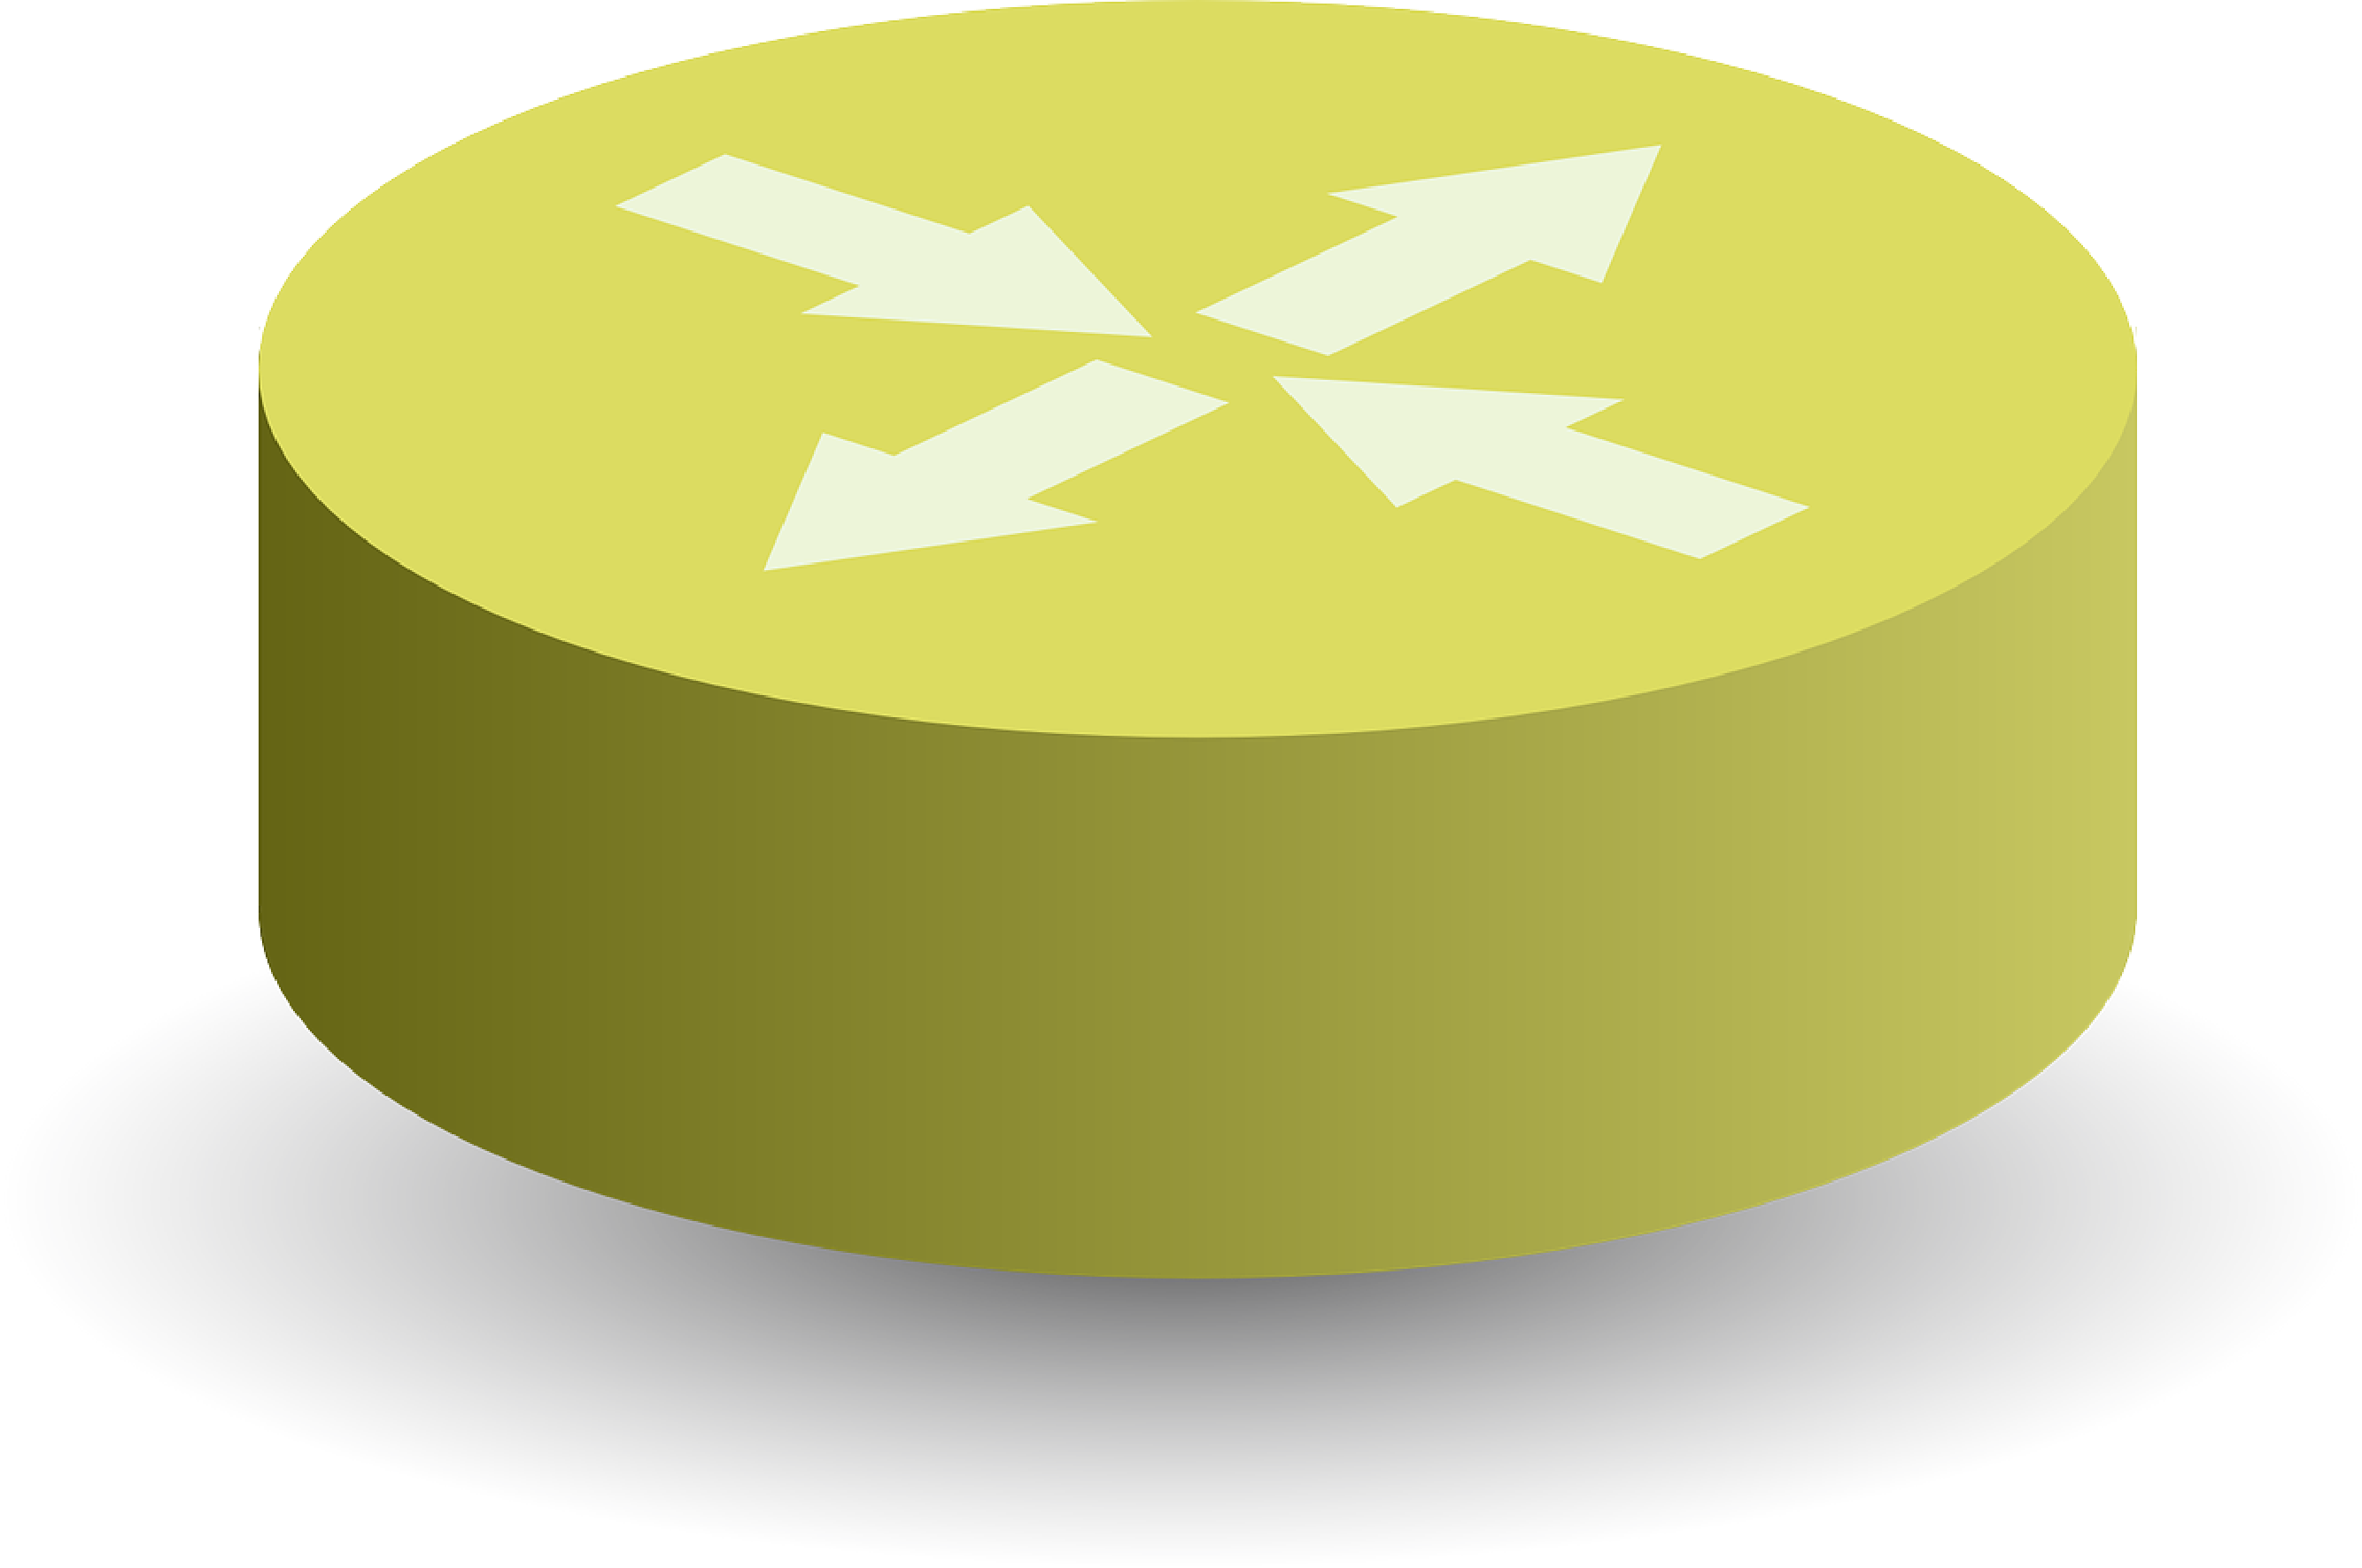
\includegraphics[width=52.5pt,height=52.5pt]{figures/router-158644_1280.pdf}};
%Image [id:dp16387001457338324] 
\draw (177.5,118) node  {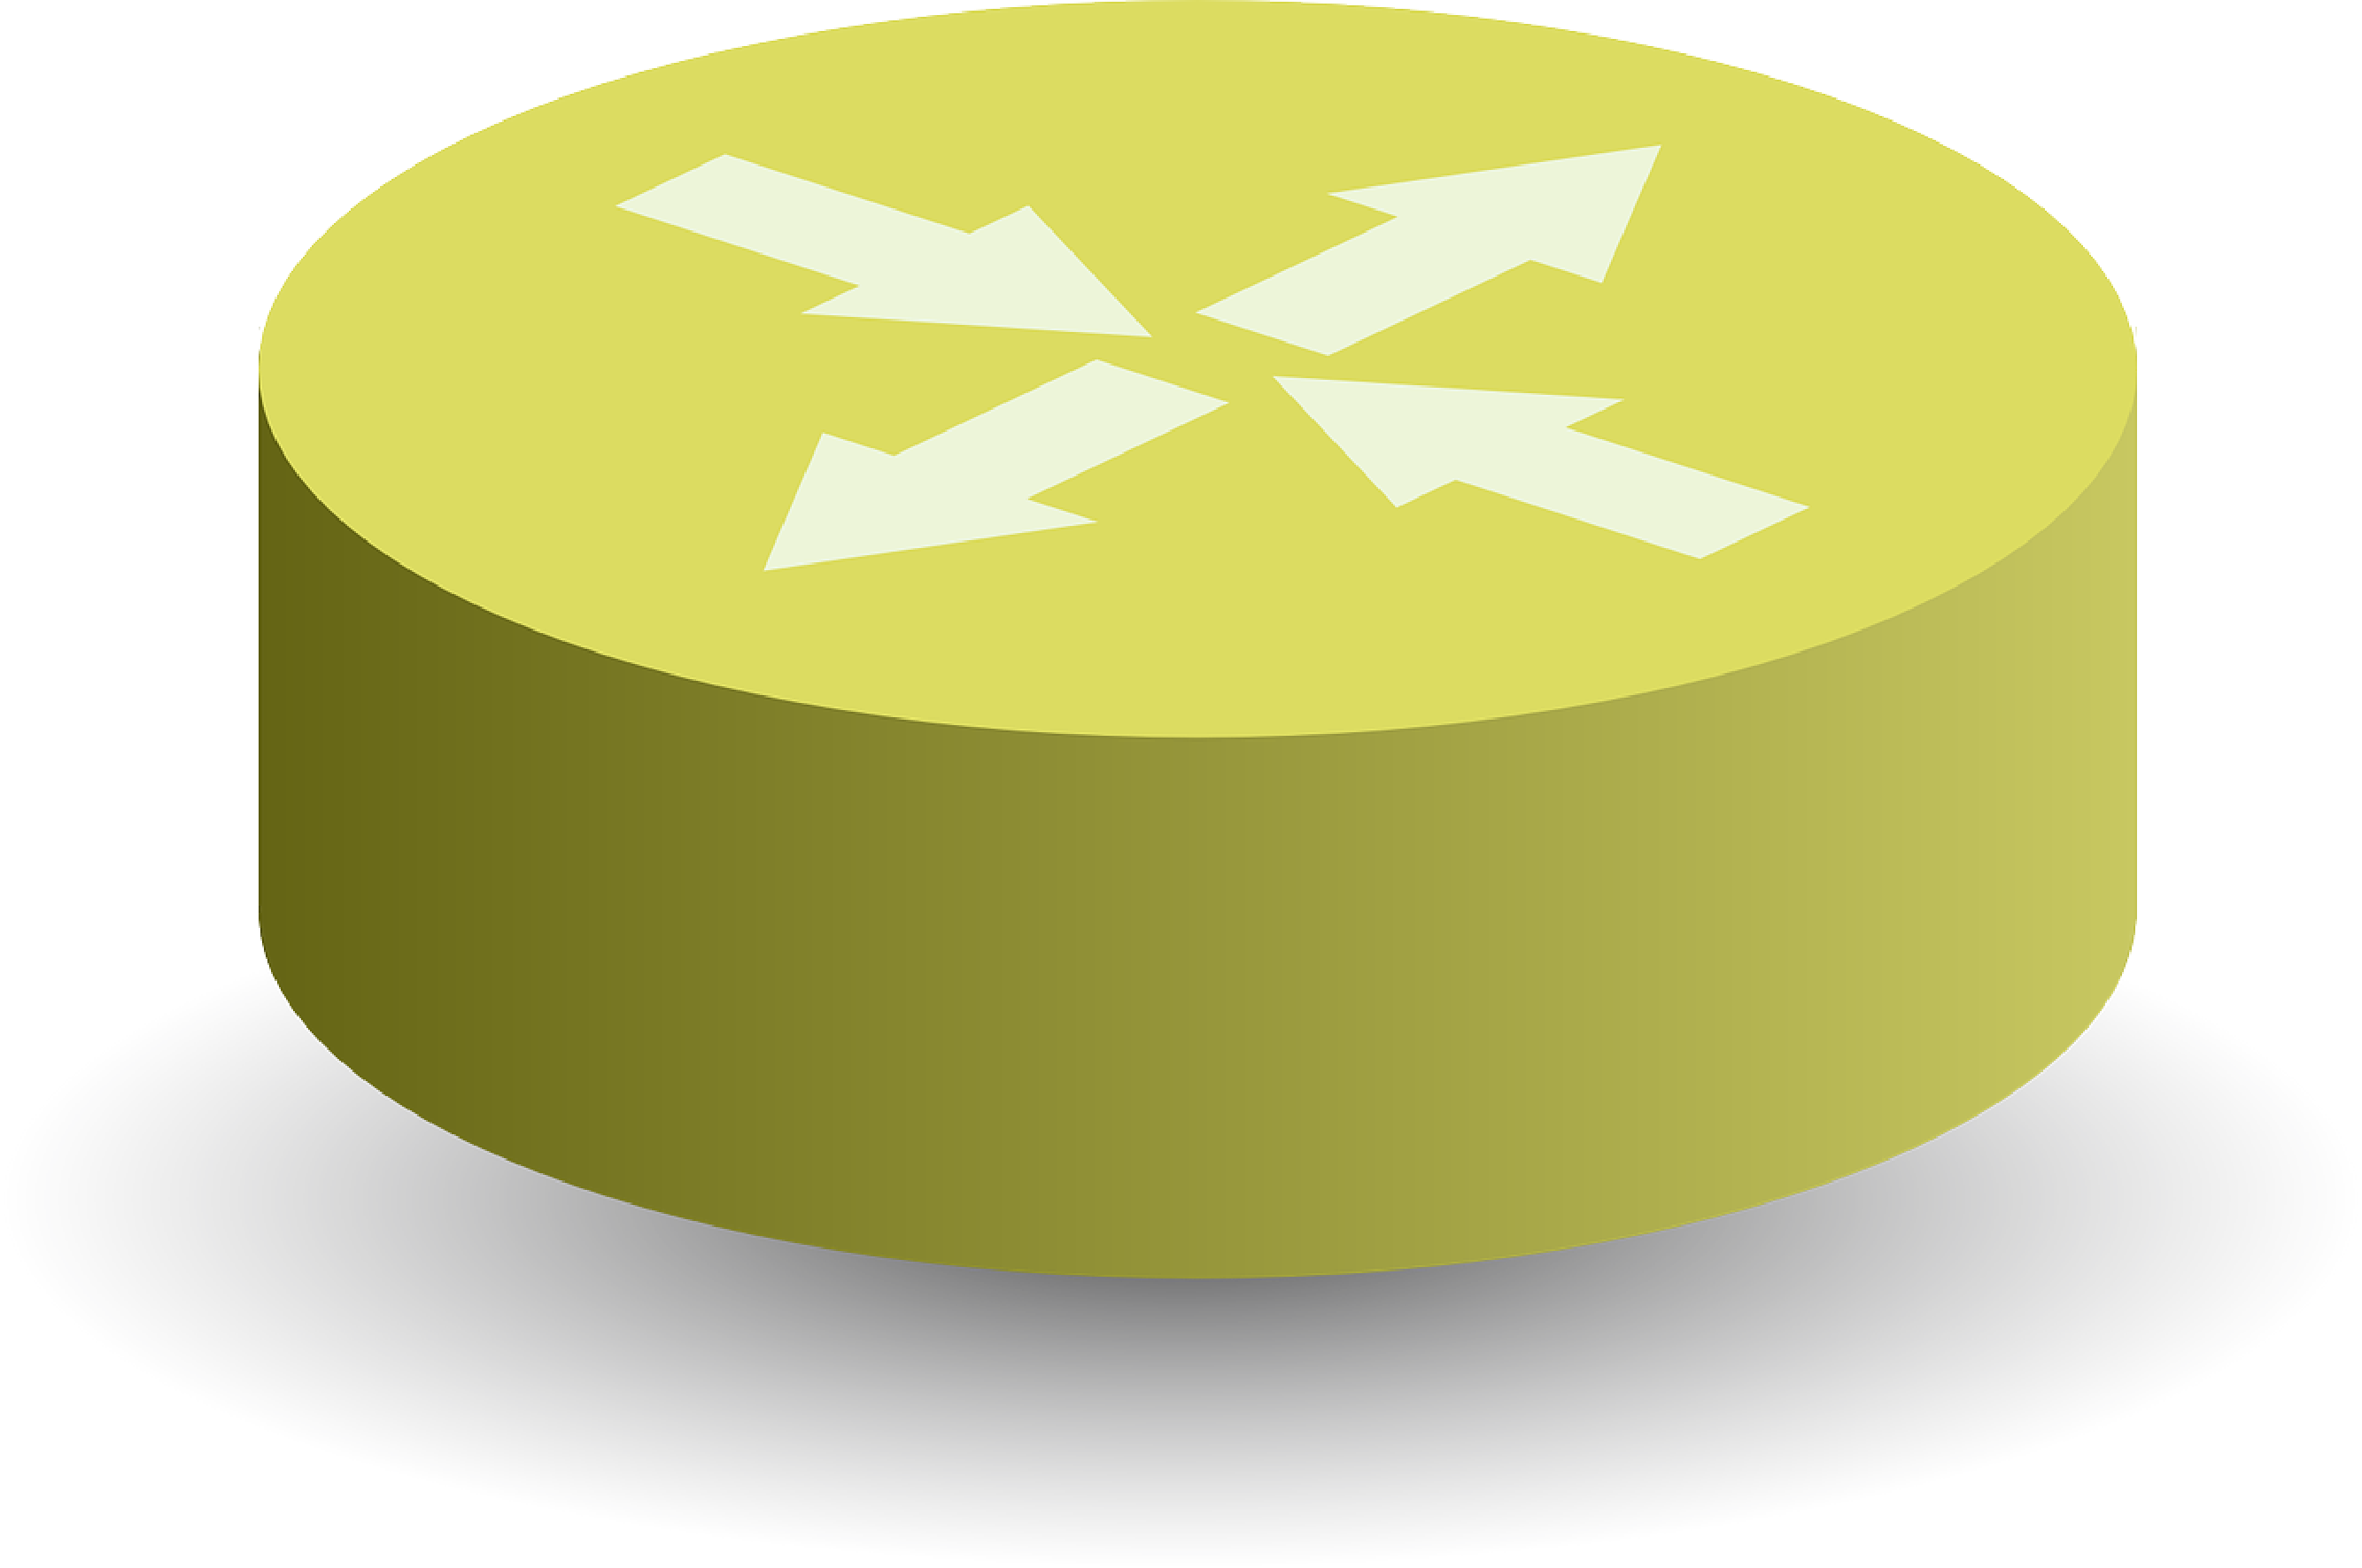
\includegraphics[width=52.5pt,height=52.5pt]{figures/router-158644_1280.pdf}};
%Image [id:dp1012276528015783] 
\draw (111.5,209.5) node  {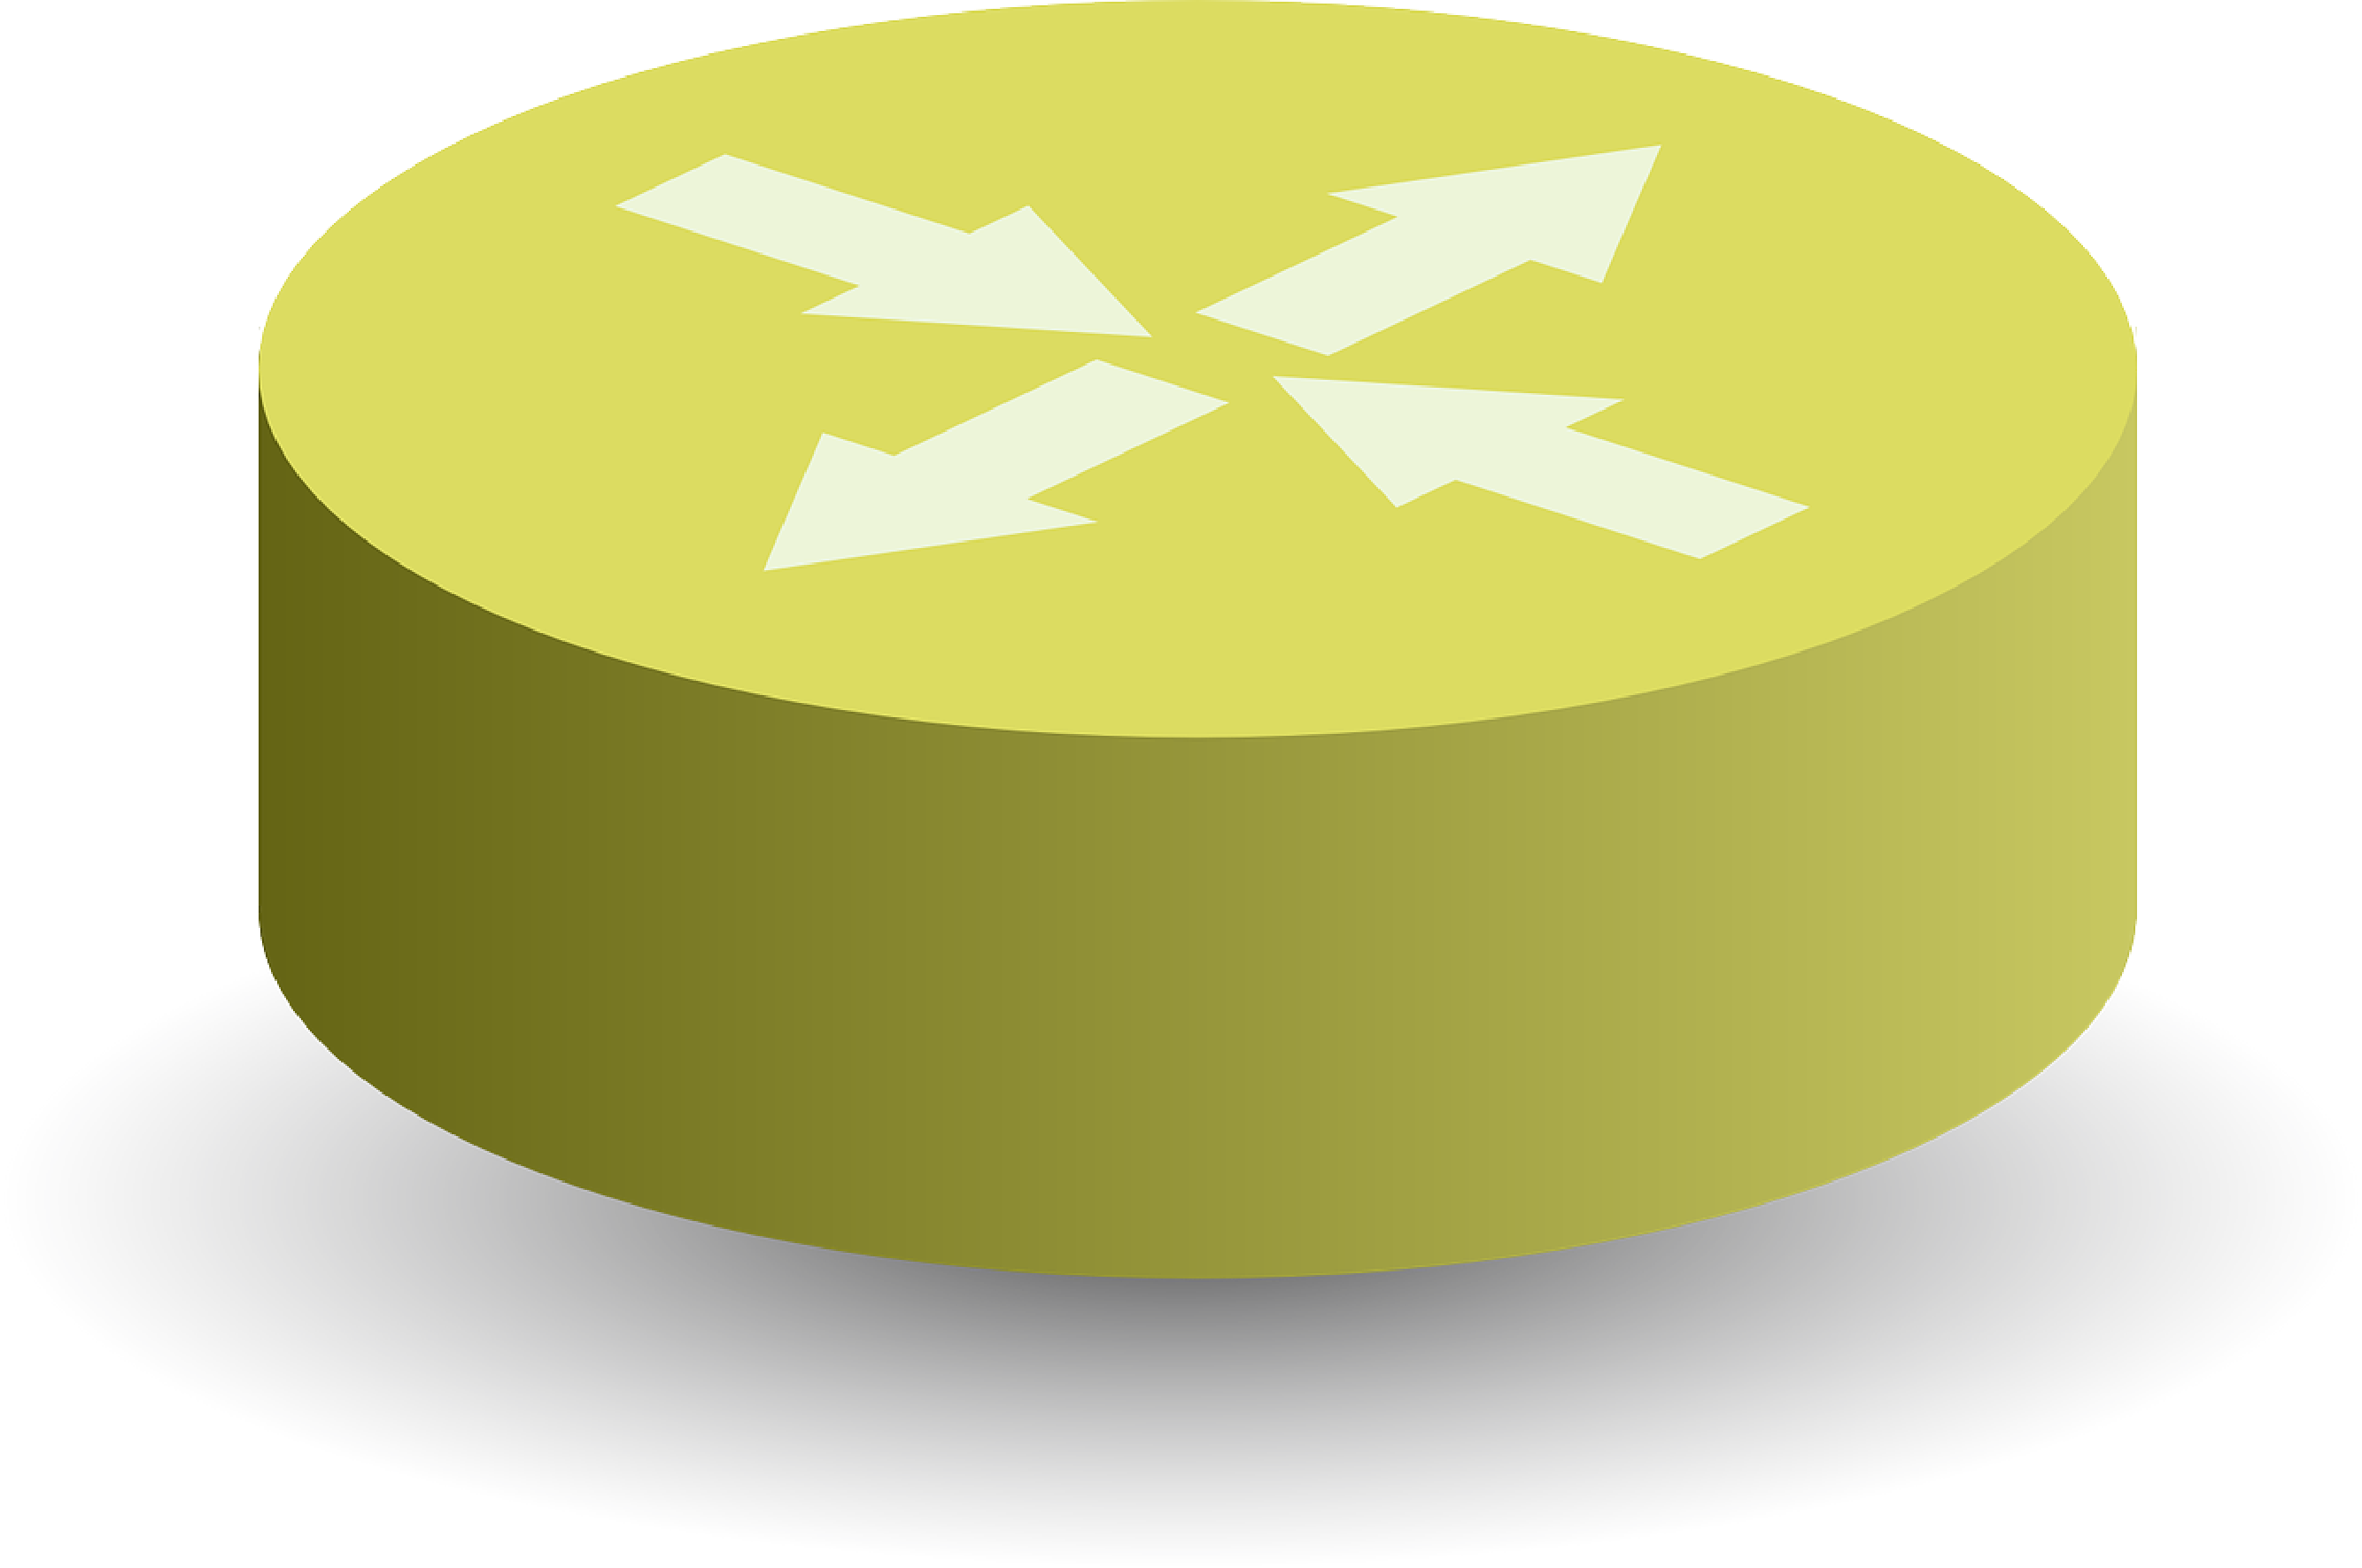
\includegraphics[width=52.5pt,height=52.5pt]{figures/router-158644_1280.pdf}};
%Straight Lines [id:da10827340921387374] 
\draw    (67,469.33) -- (180,428.33) ;


%Straight Lines [id:da02465044628511004] 
\draw    (67,469.33) -- (182,526.33) ;


%Straight Lines [id:da7232328020483667] 
\draw    (179,526.33) -- (177,428.33) ;


%Straight Lines [id:da6335138571596731] 
\draw    (440,530.33) -- (438,432.33) ;


%Straight Lines [id:da5081473547182844] 
\draw    (186,435.33) -- (462,436.33) ;


%Straight Lines [id:da5273919871085183] 
\draw    (185,530.33) -- (461,531.33) ;


%Image [id:dp10904051335047615] 
\draw (68,484.5) node  {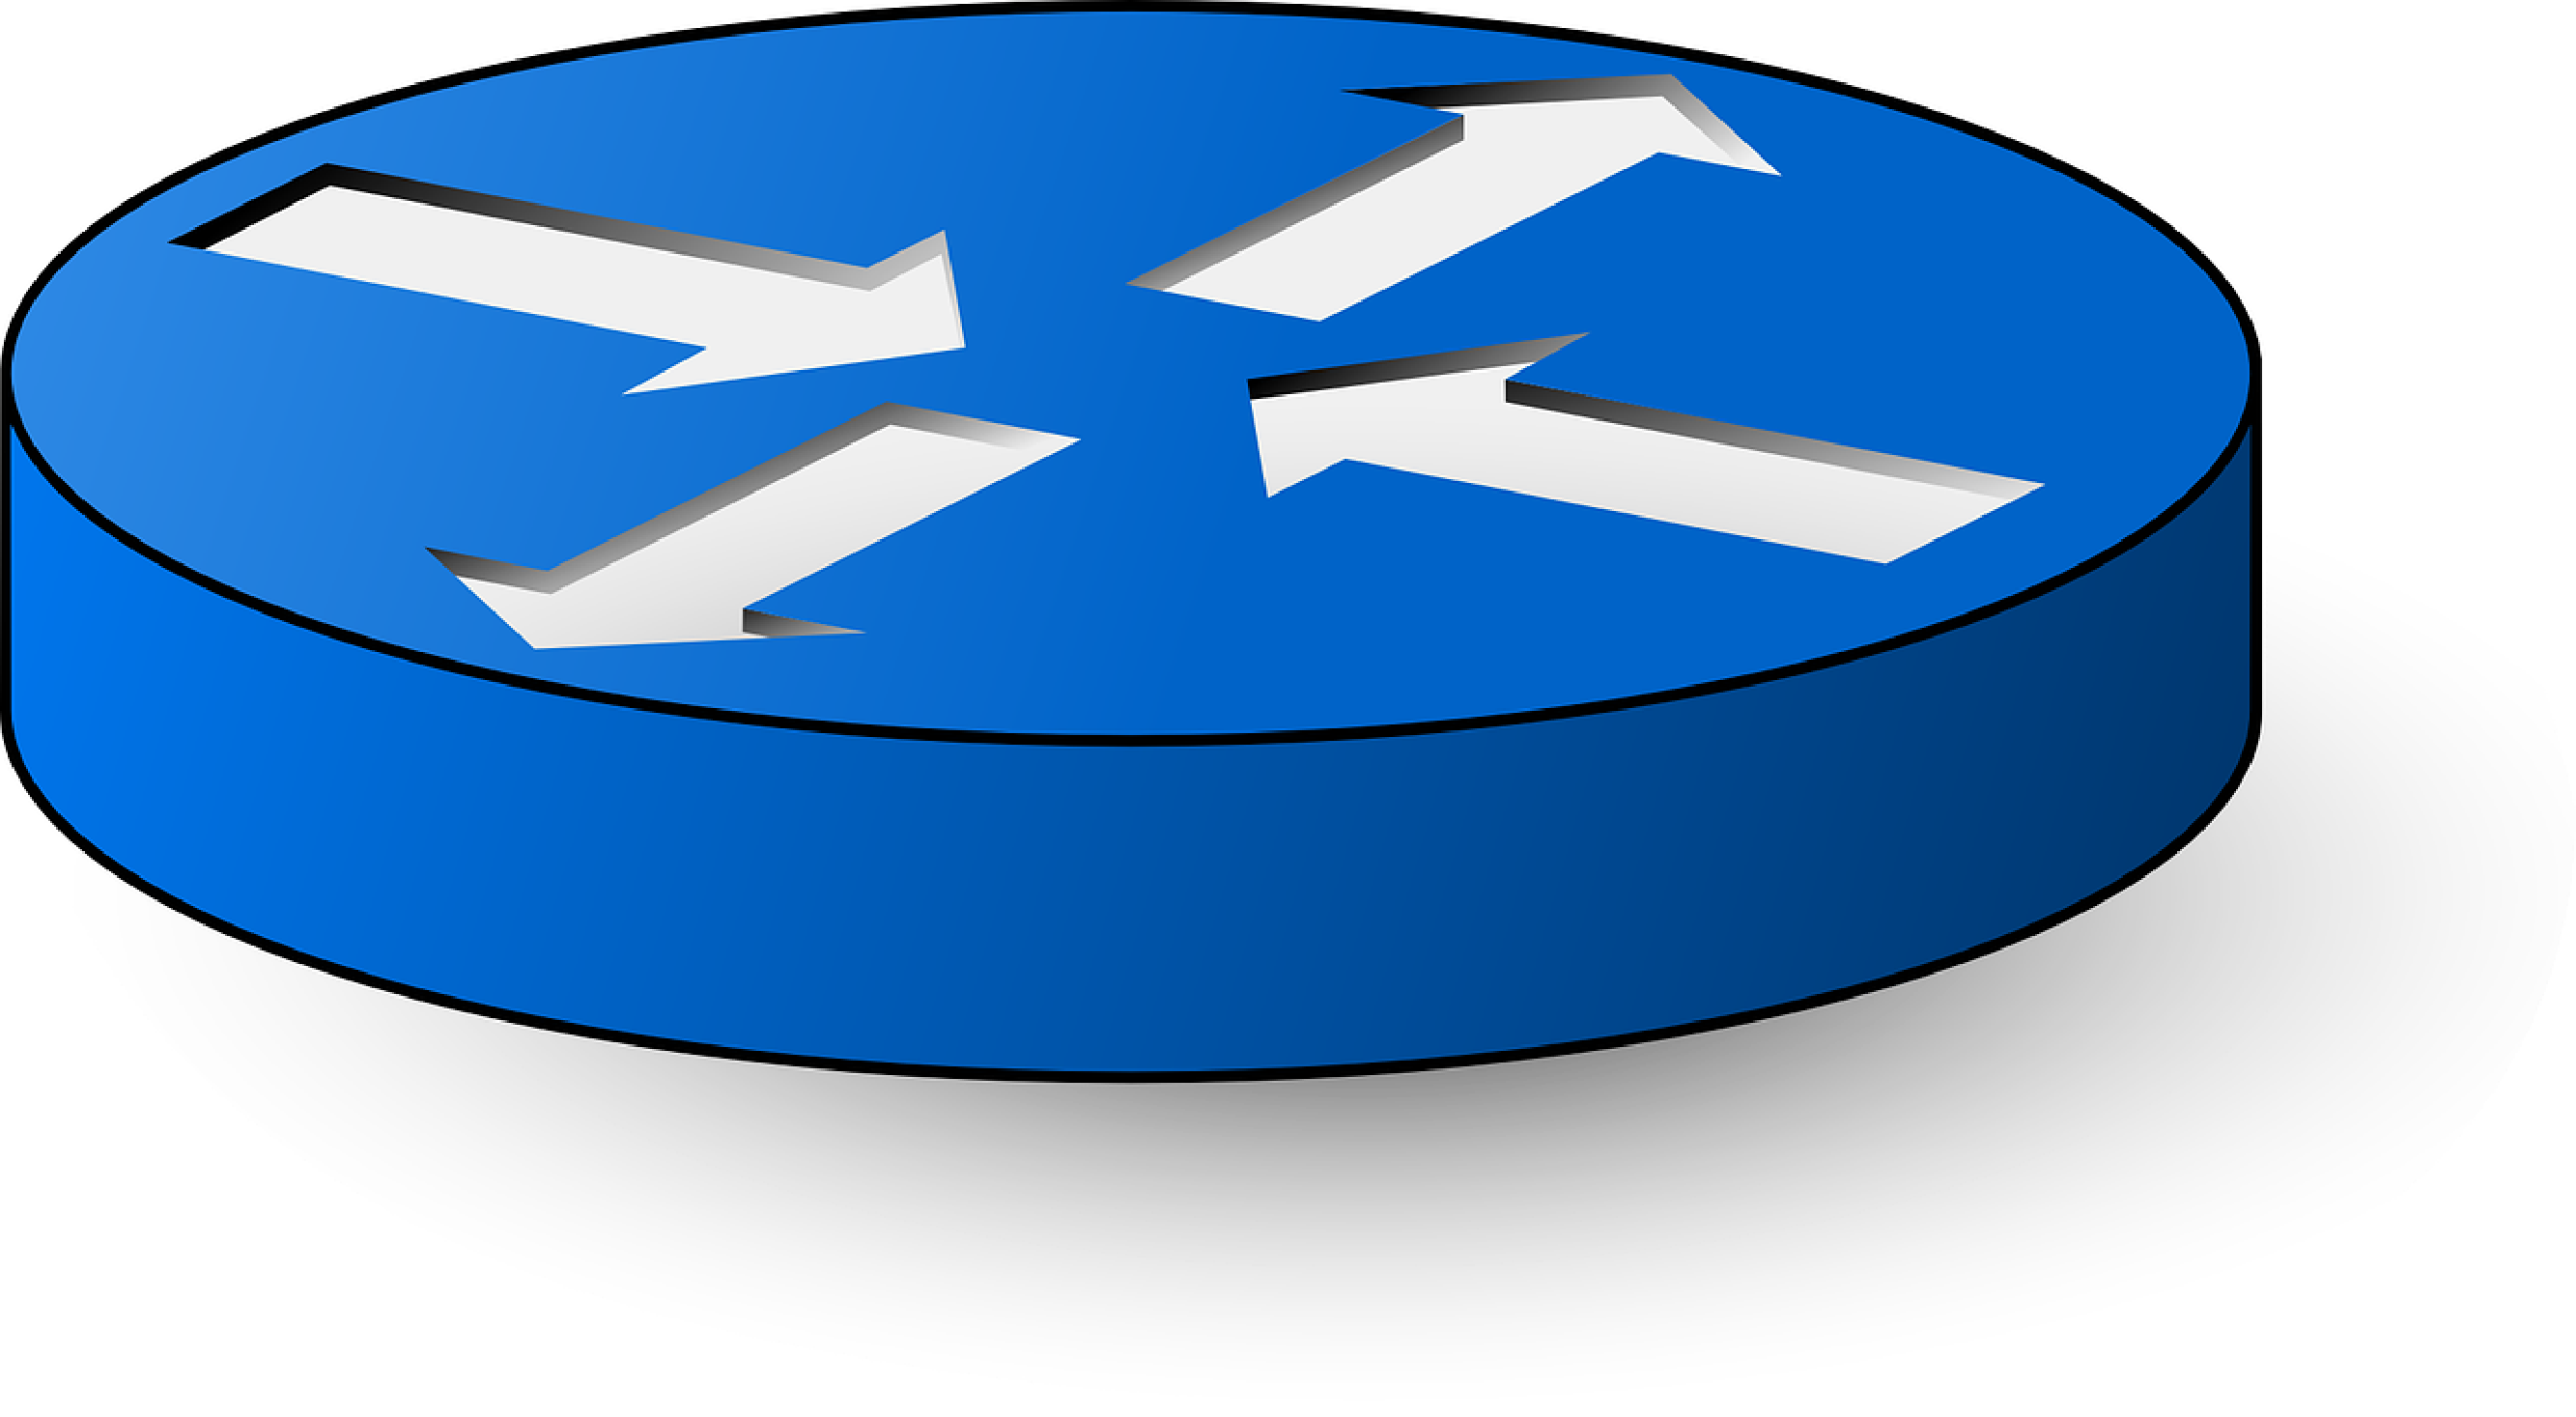
\includegraphics[width=52.5pt,height=52.5pt]{figures/router-30140_1280.pdf}};
%Image [id:dp7146163070755307] 
\draw (185,444.5) node  {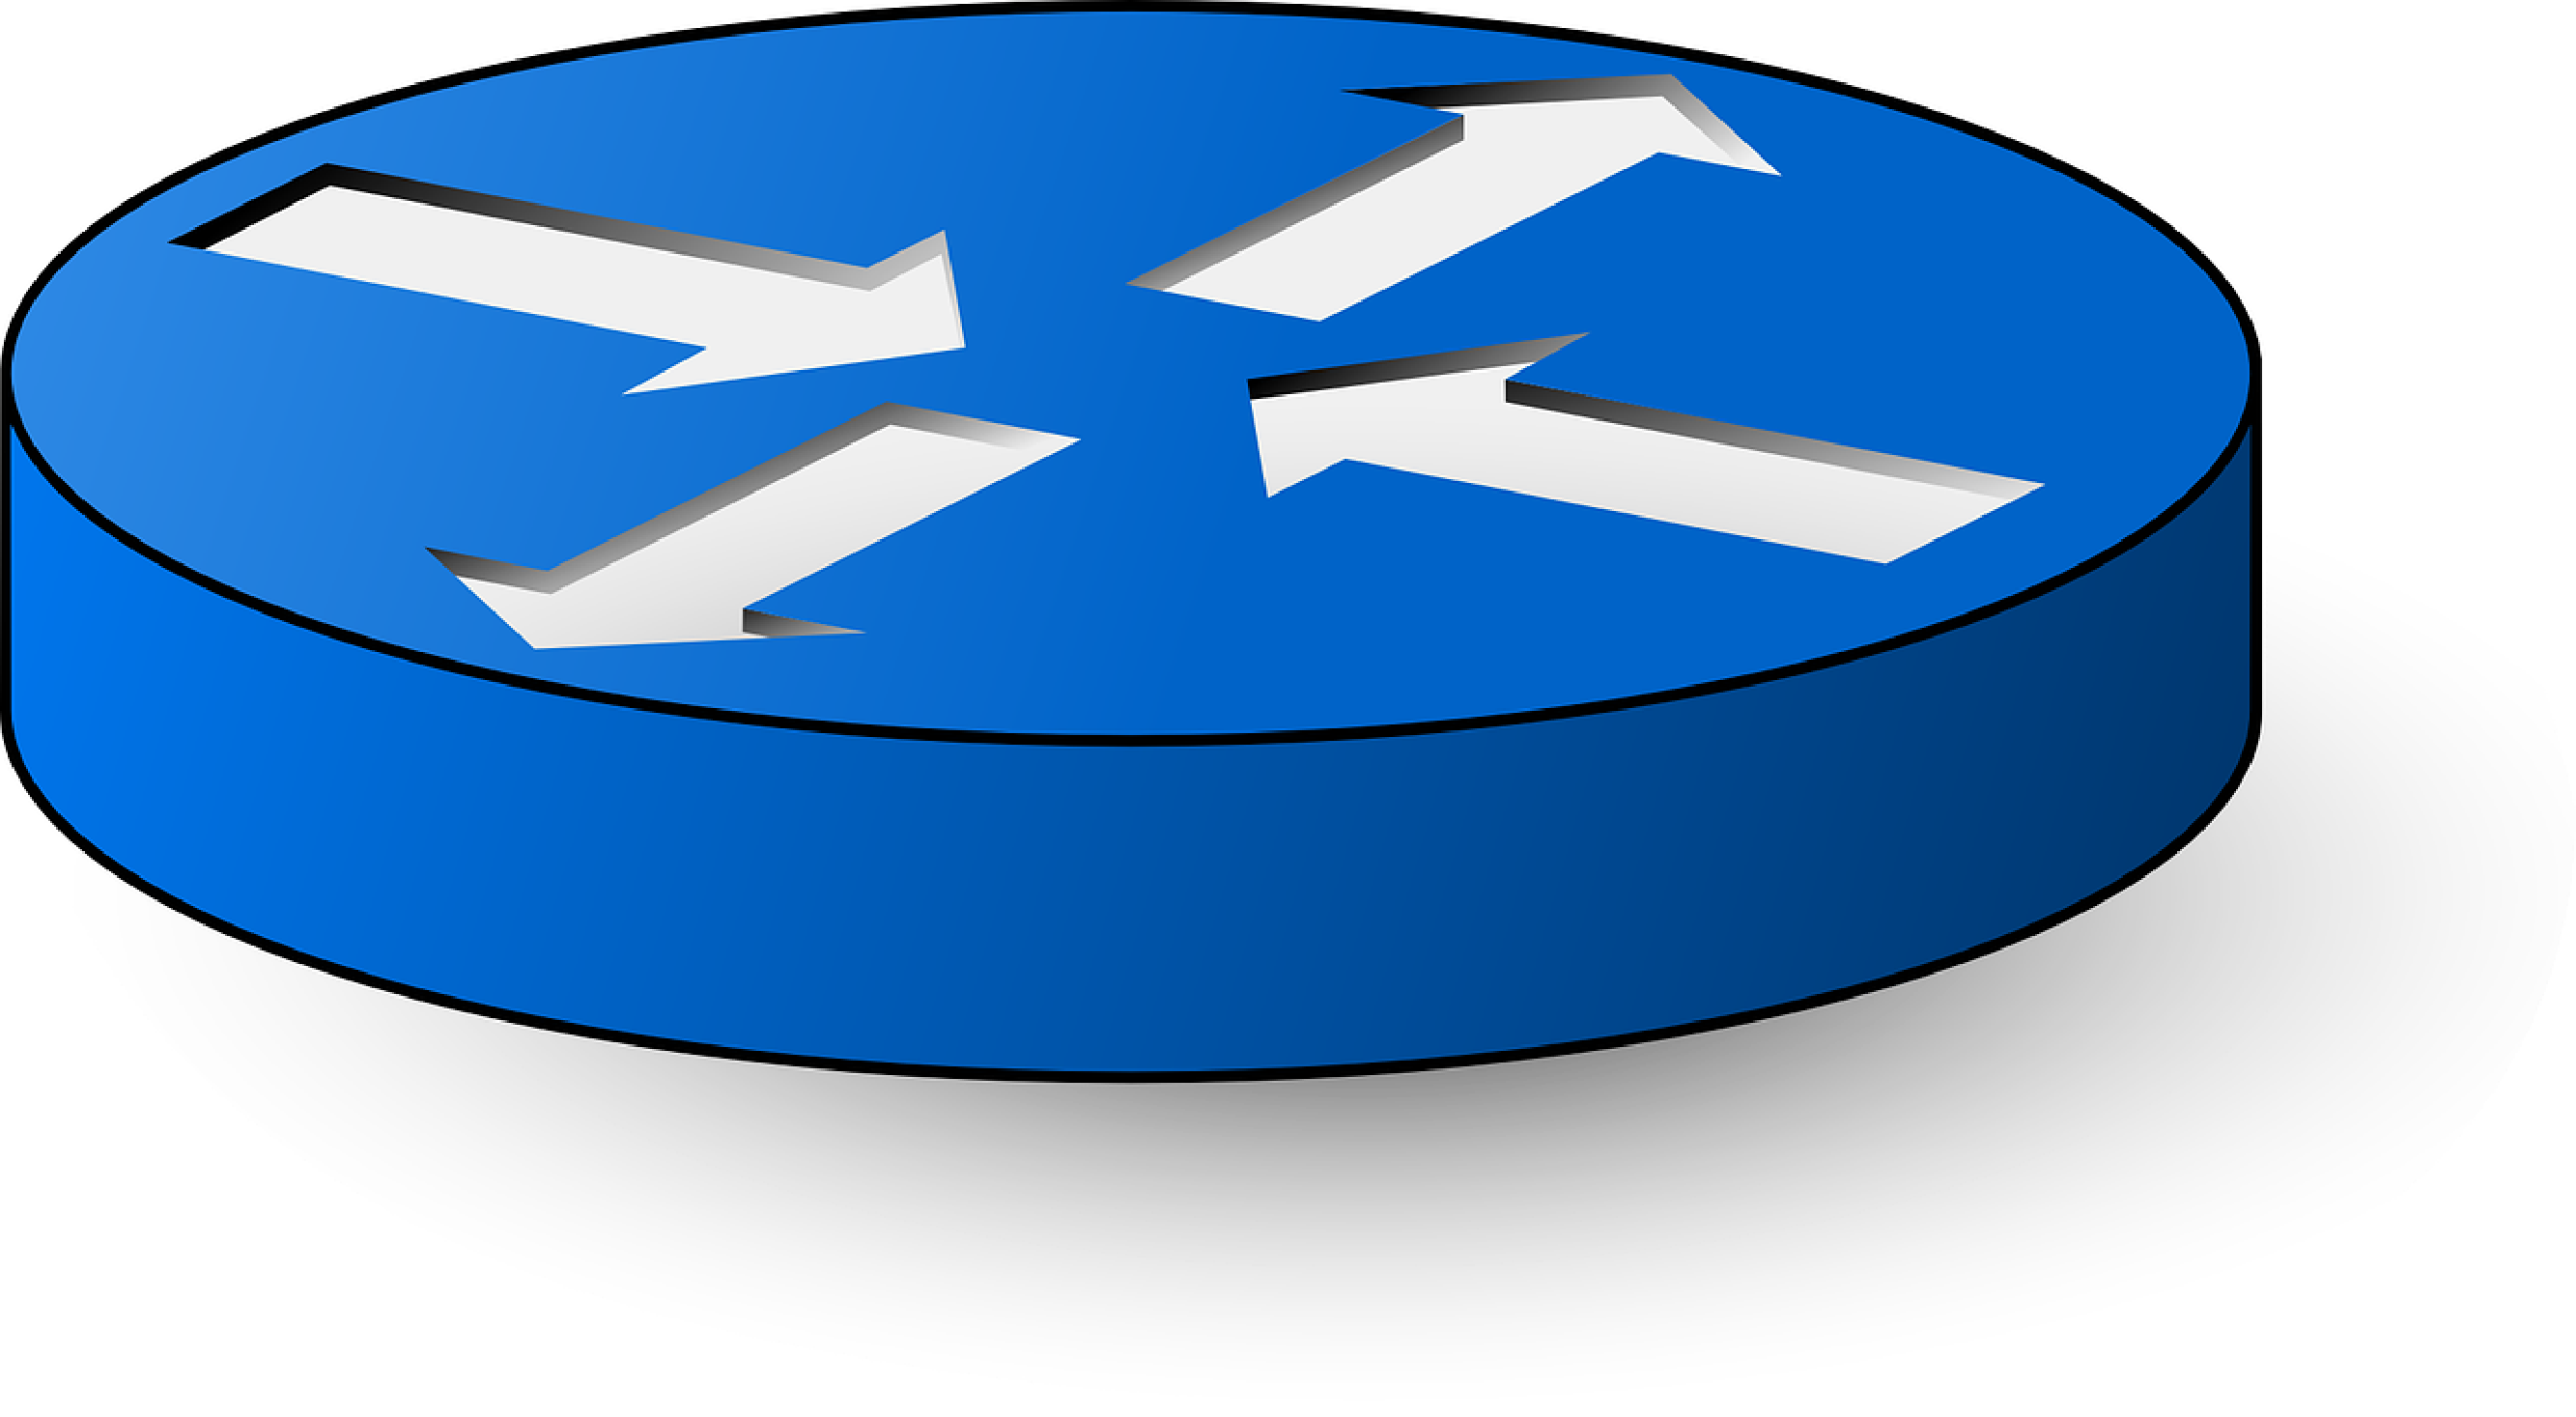
\includegraphics[width=52.5pt,height=52.5pt]{figures/router-30140_1280.pdf}};
%Image [id:dp9757131158412626] 
\draw (441.5,544.5) node  {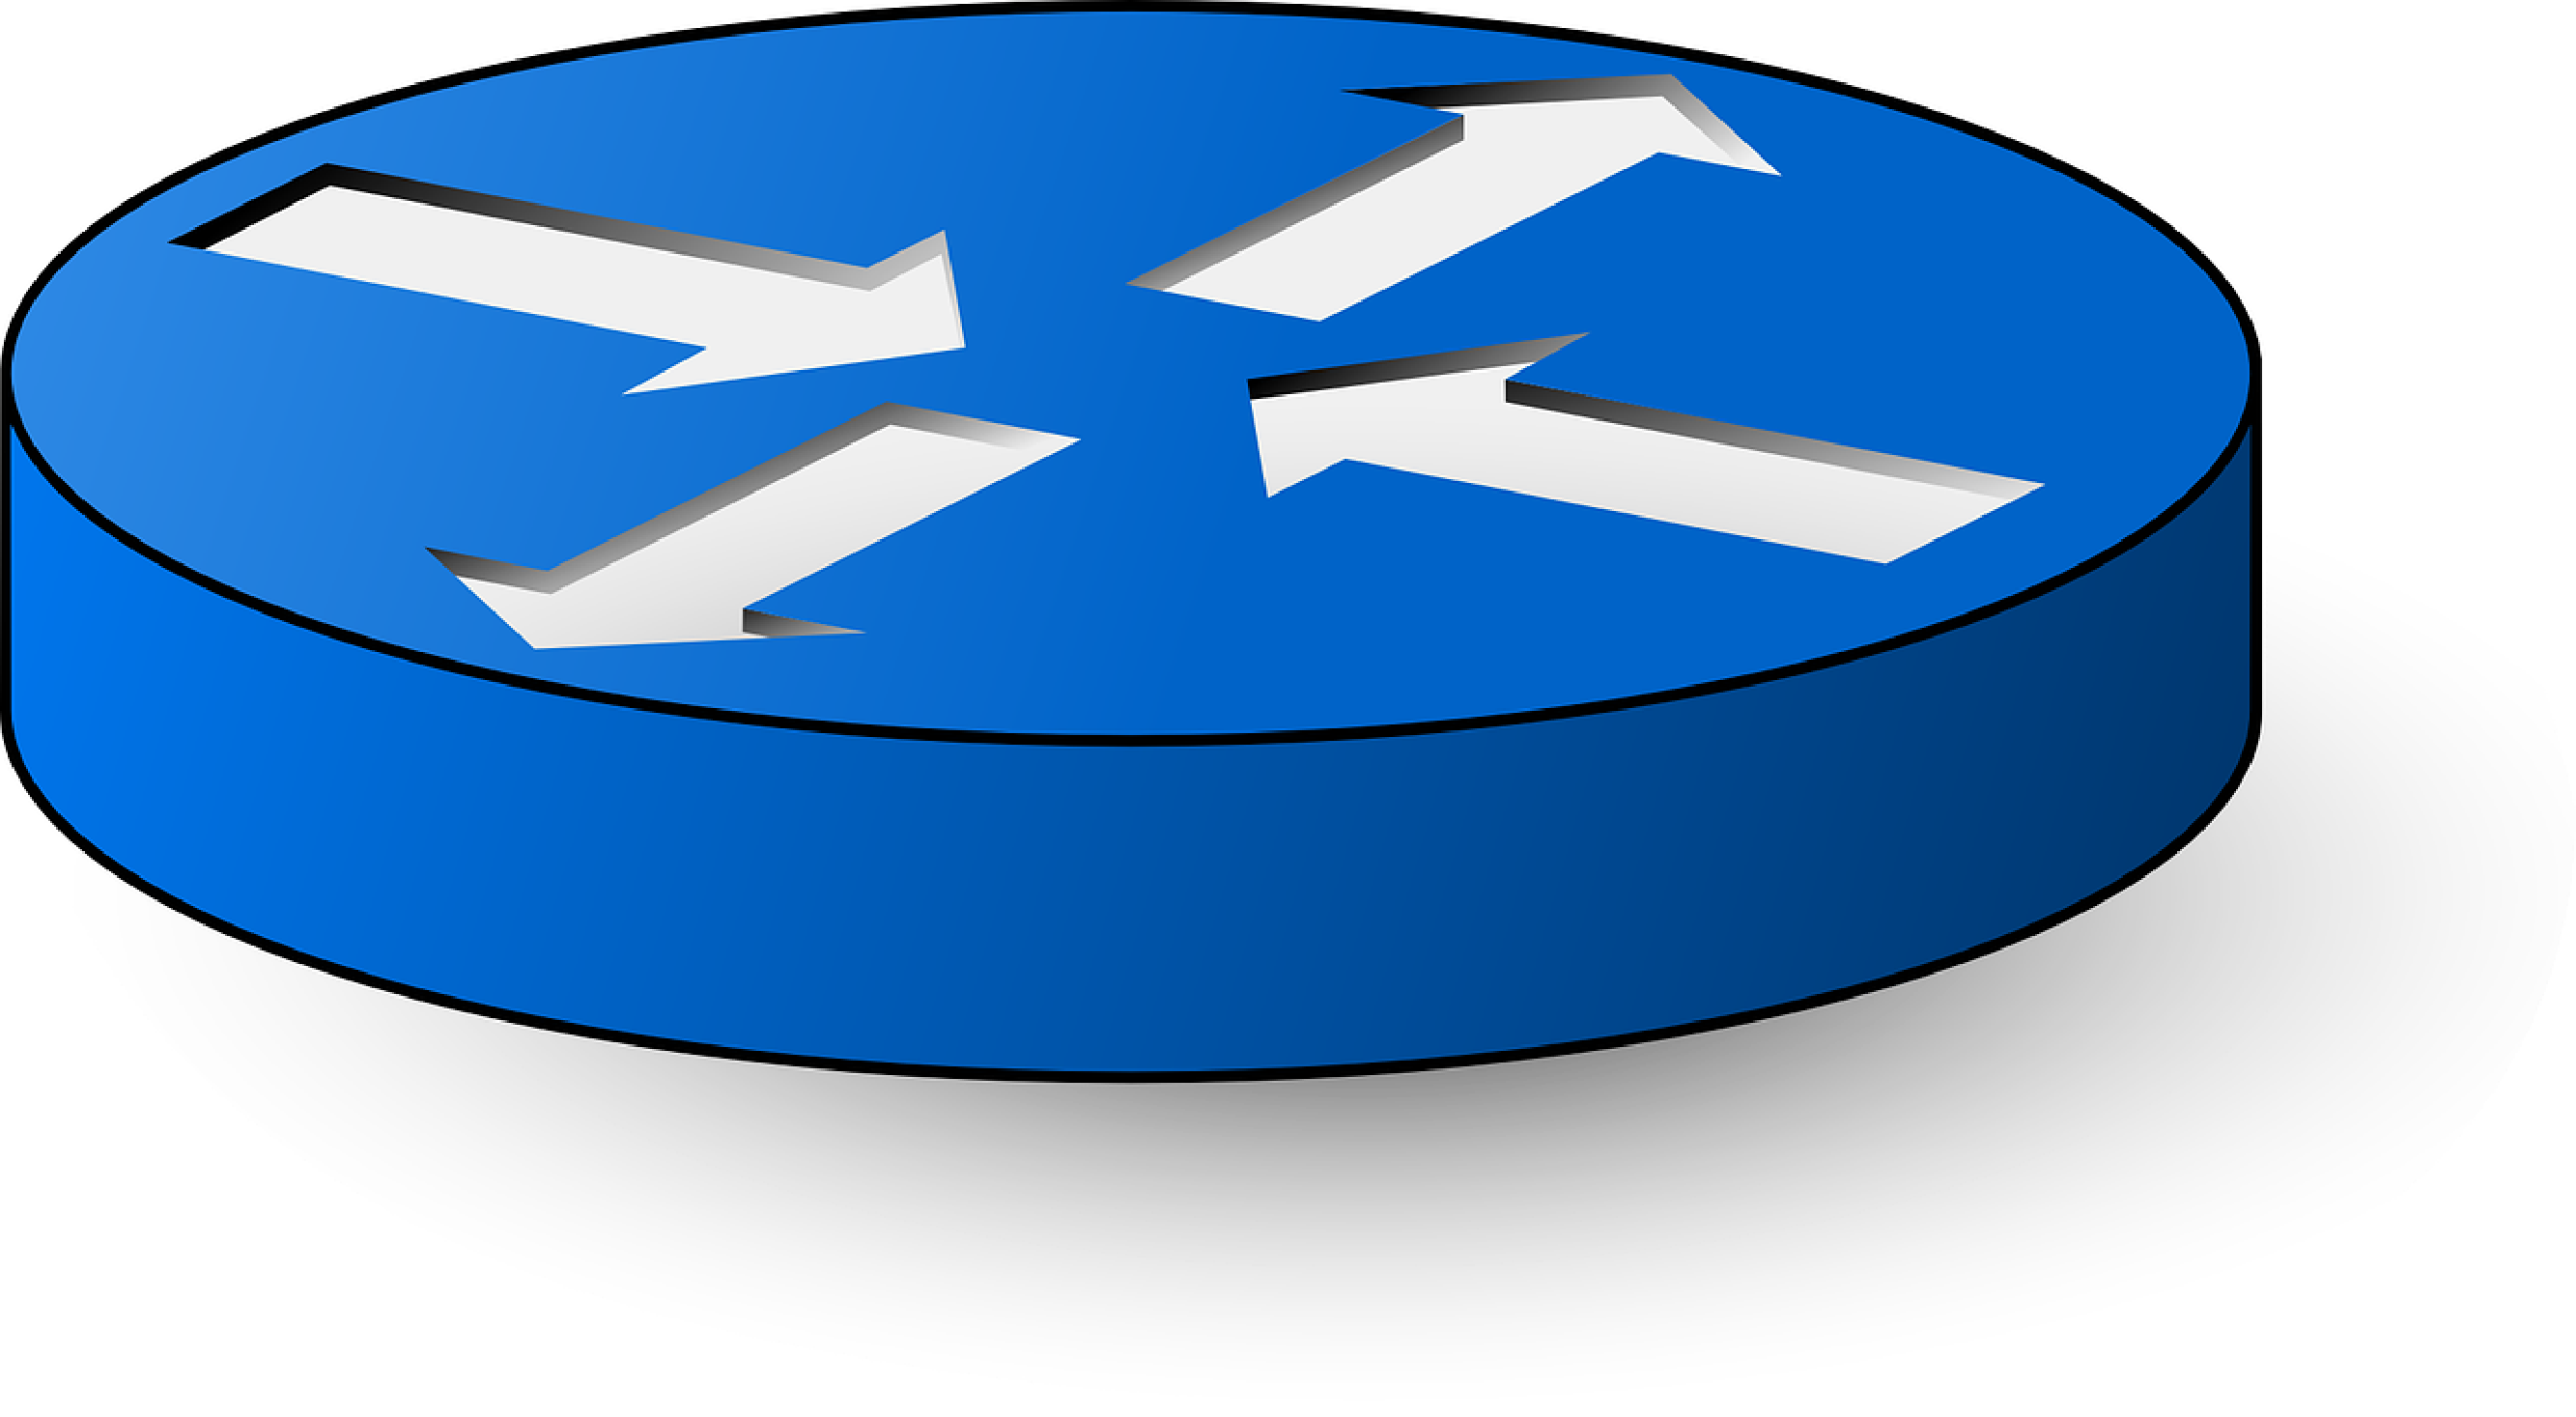
\includegraphics[width=52.5pt,height=52.5pt]{figures/router-30140_1280.pdf}};
%Image [id:dp21403253894649854] 
\draw (184,546.5) node  {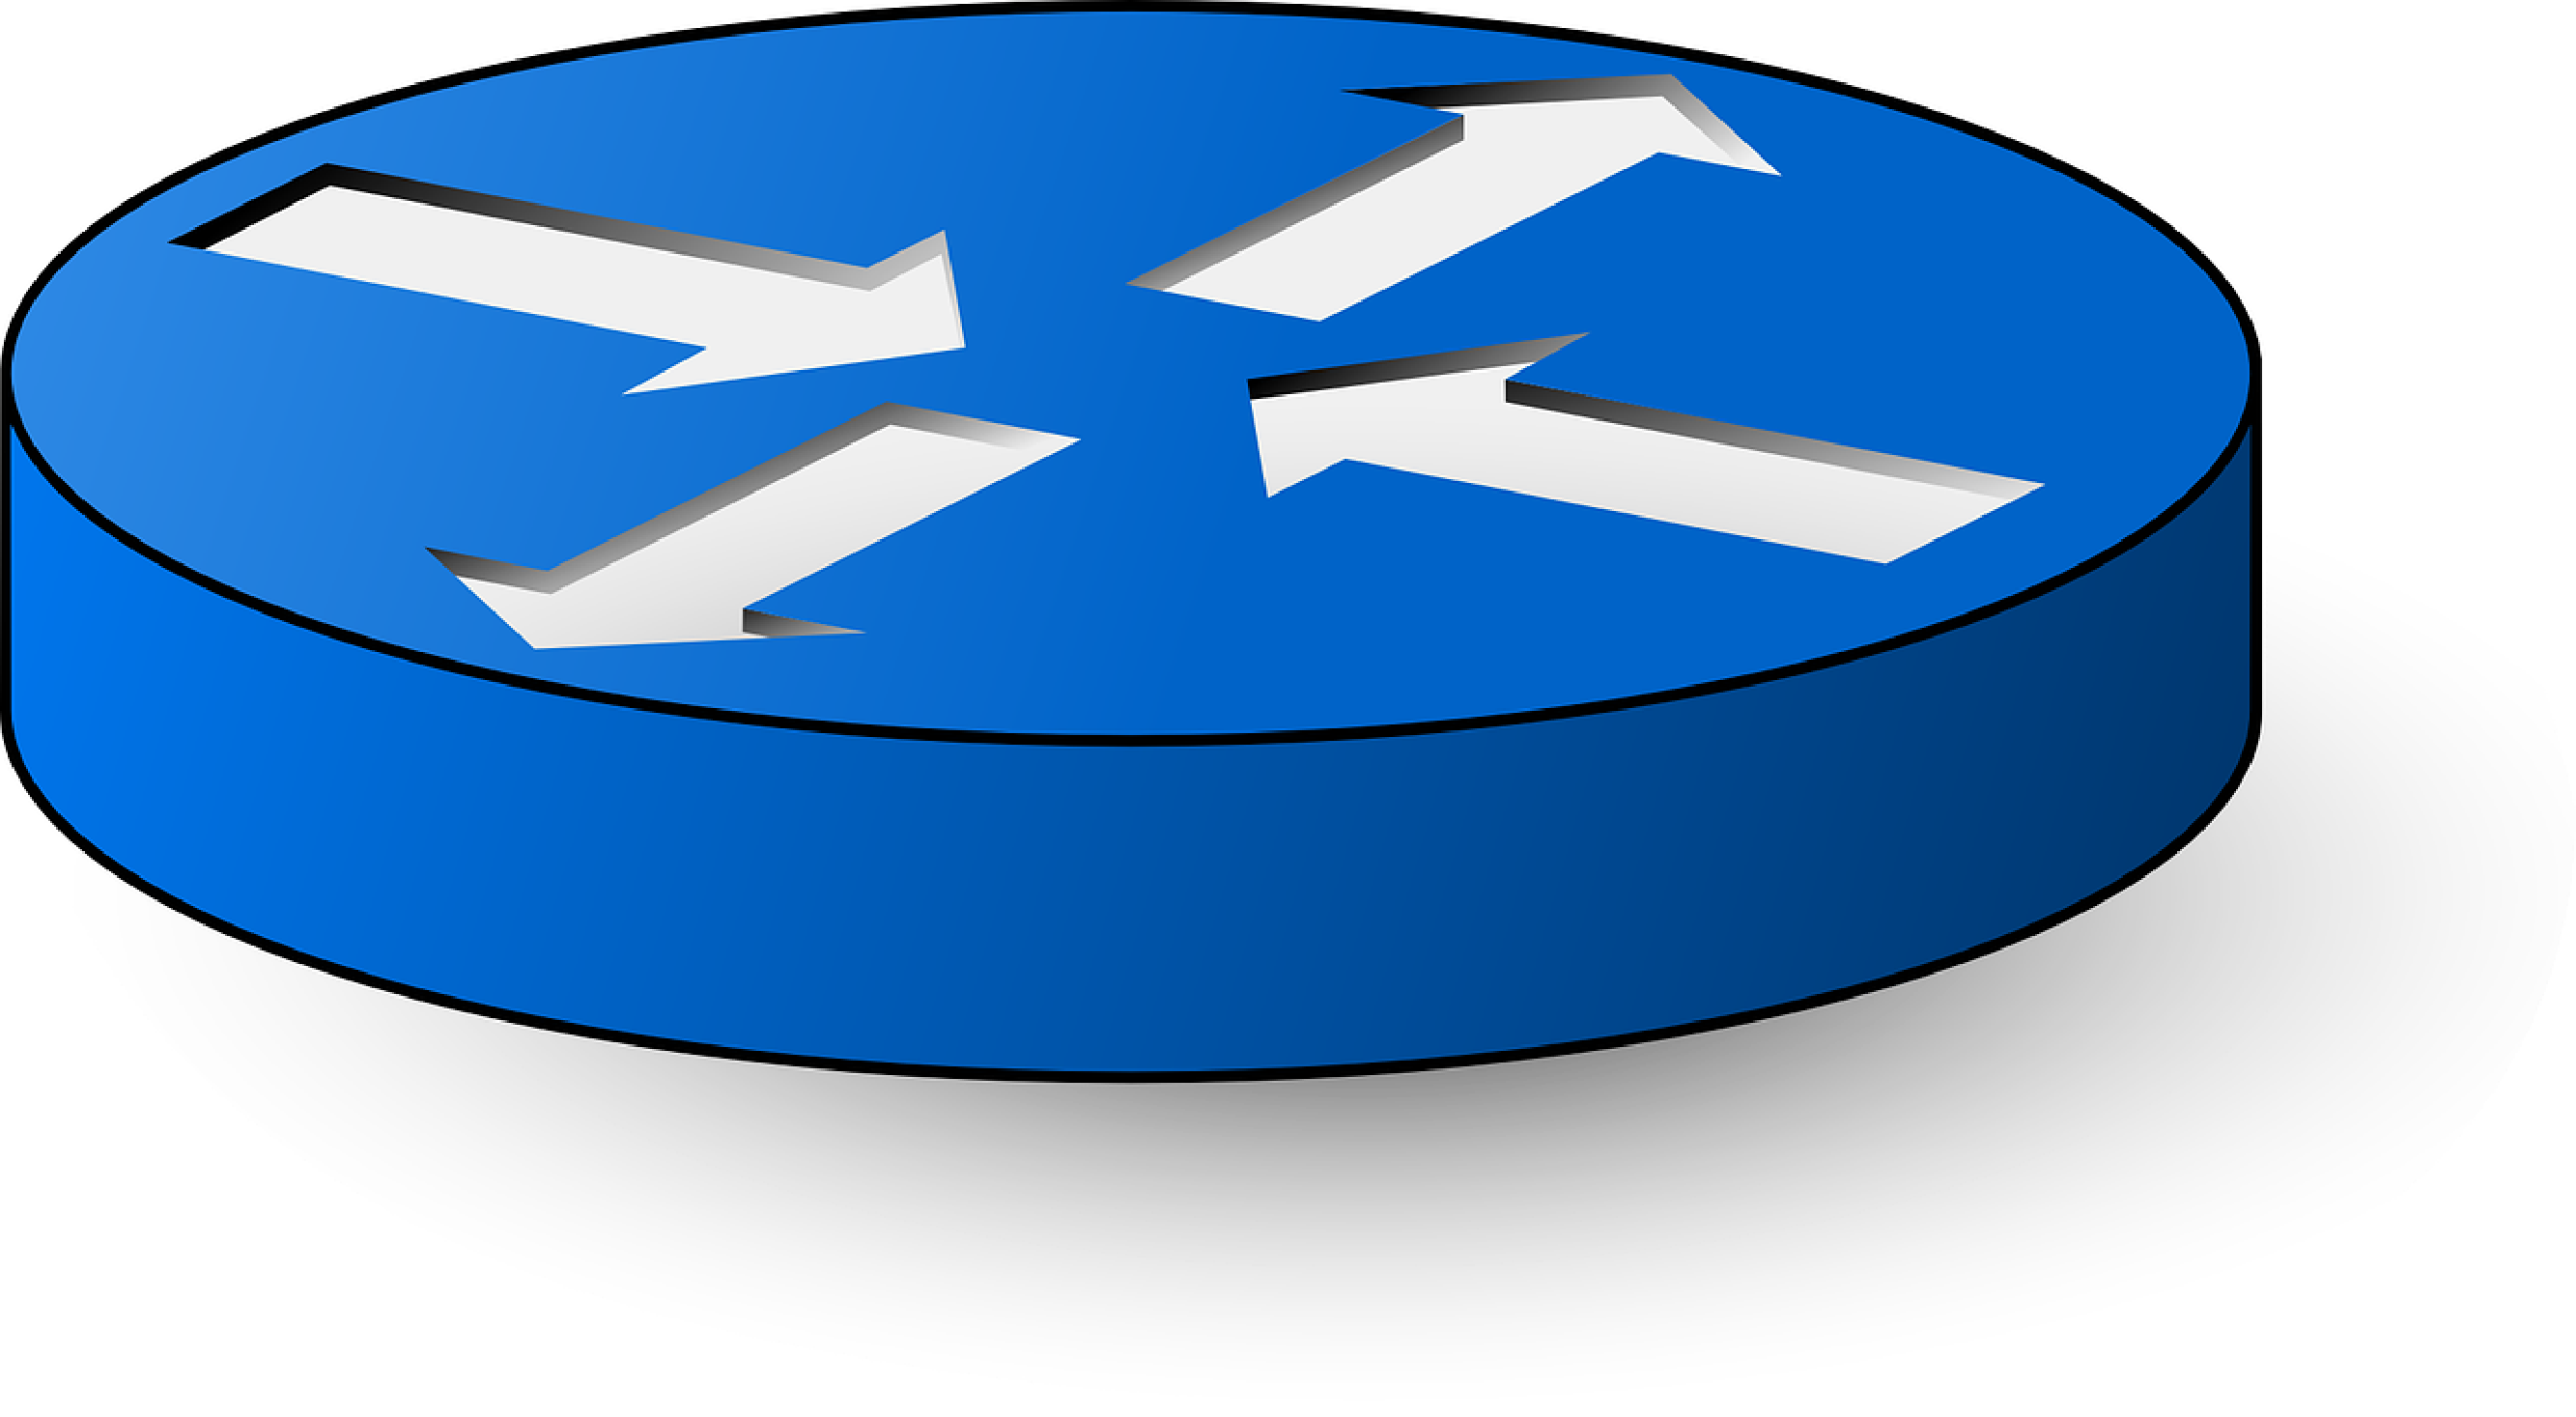
\includegraphics[width=52.5pt,height=52.5pt]{figures/router-30140_1280.pdf}};
%Image [id:dp9442712298825287] 
\draw (440.5,444.5) node  {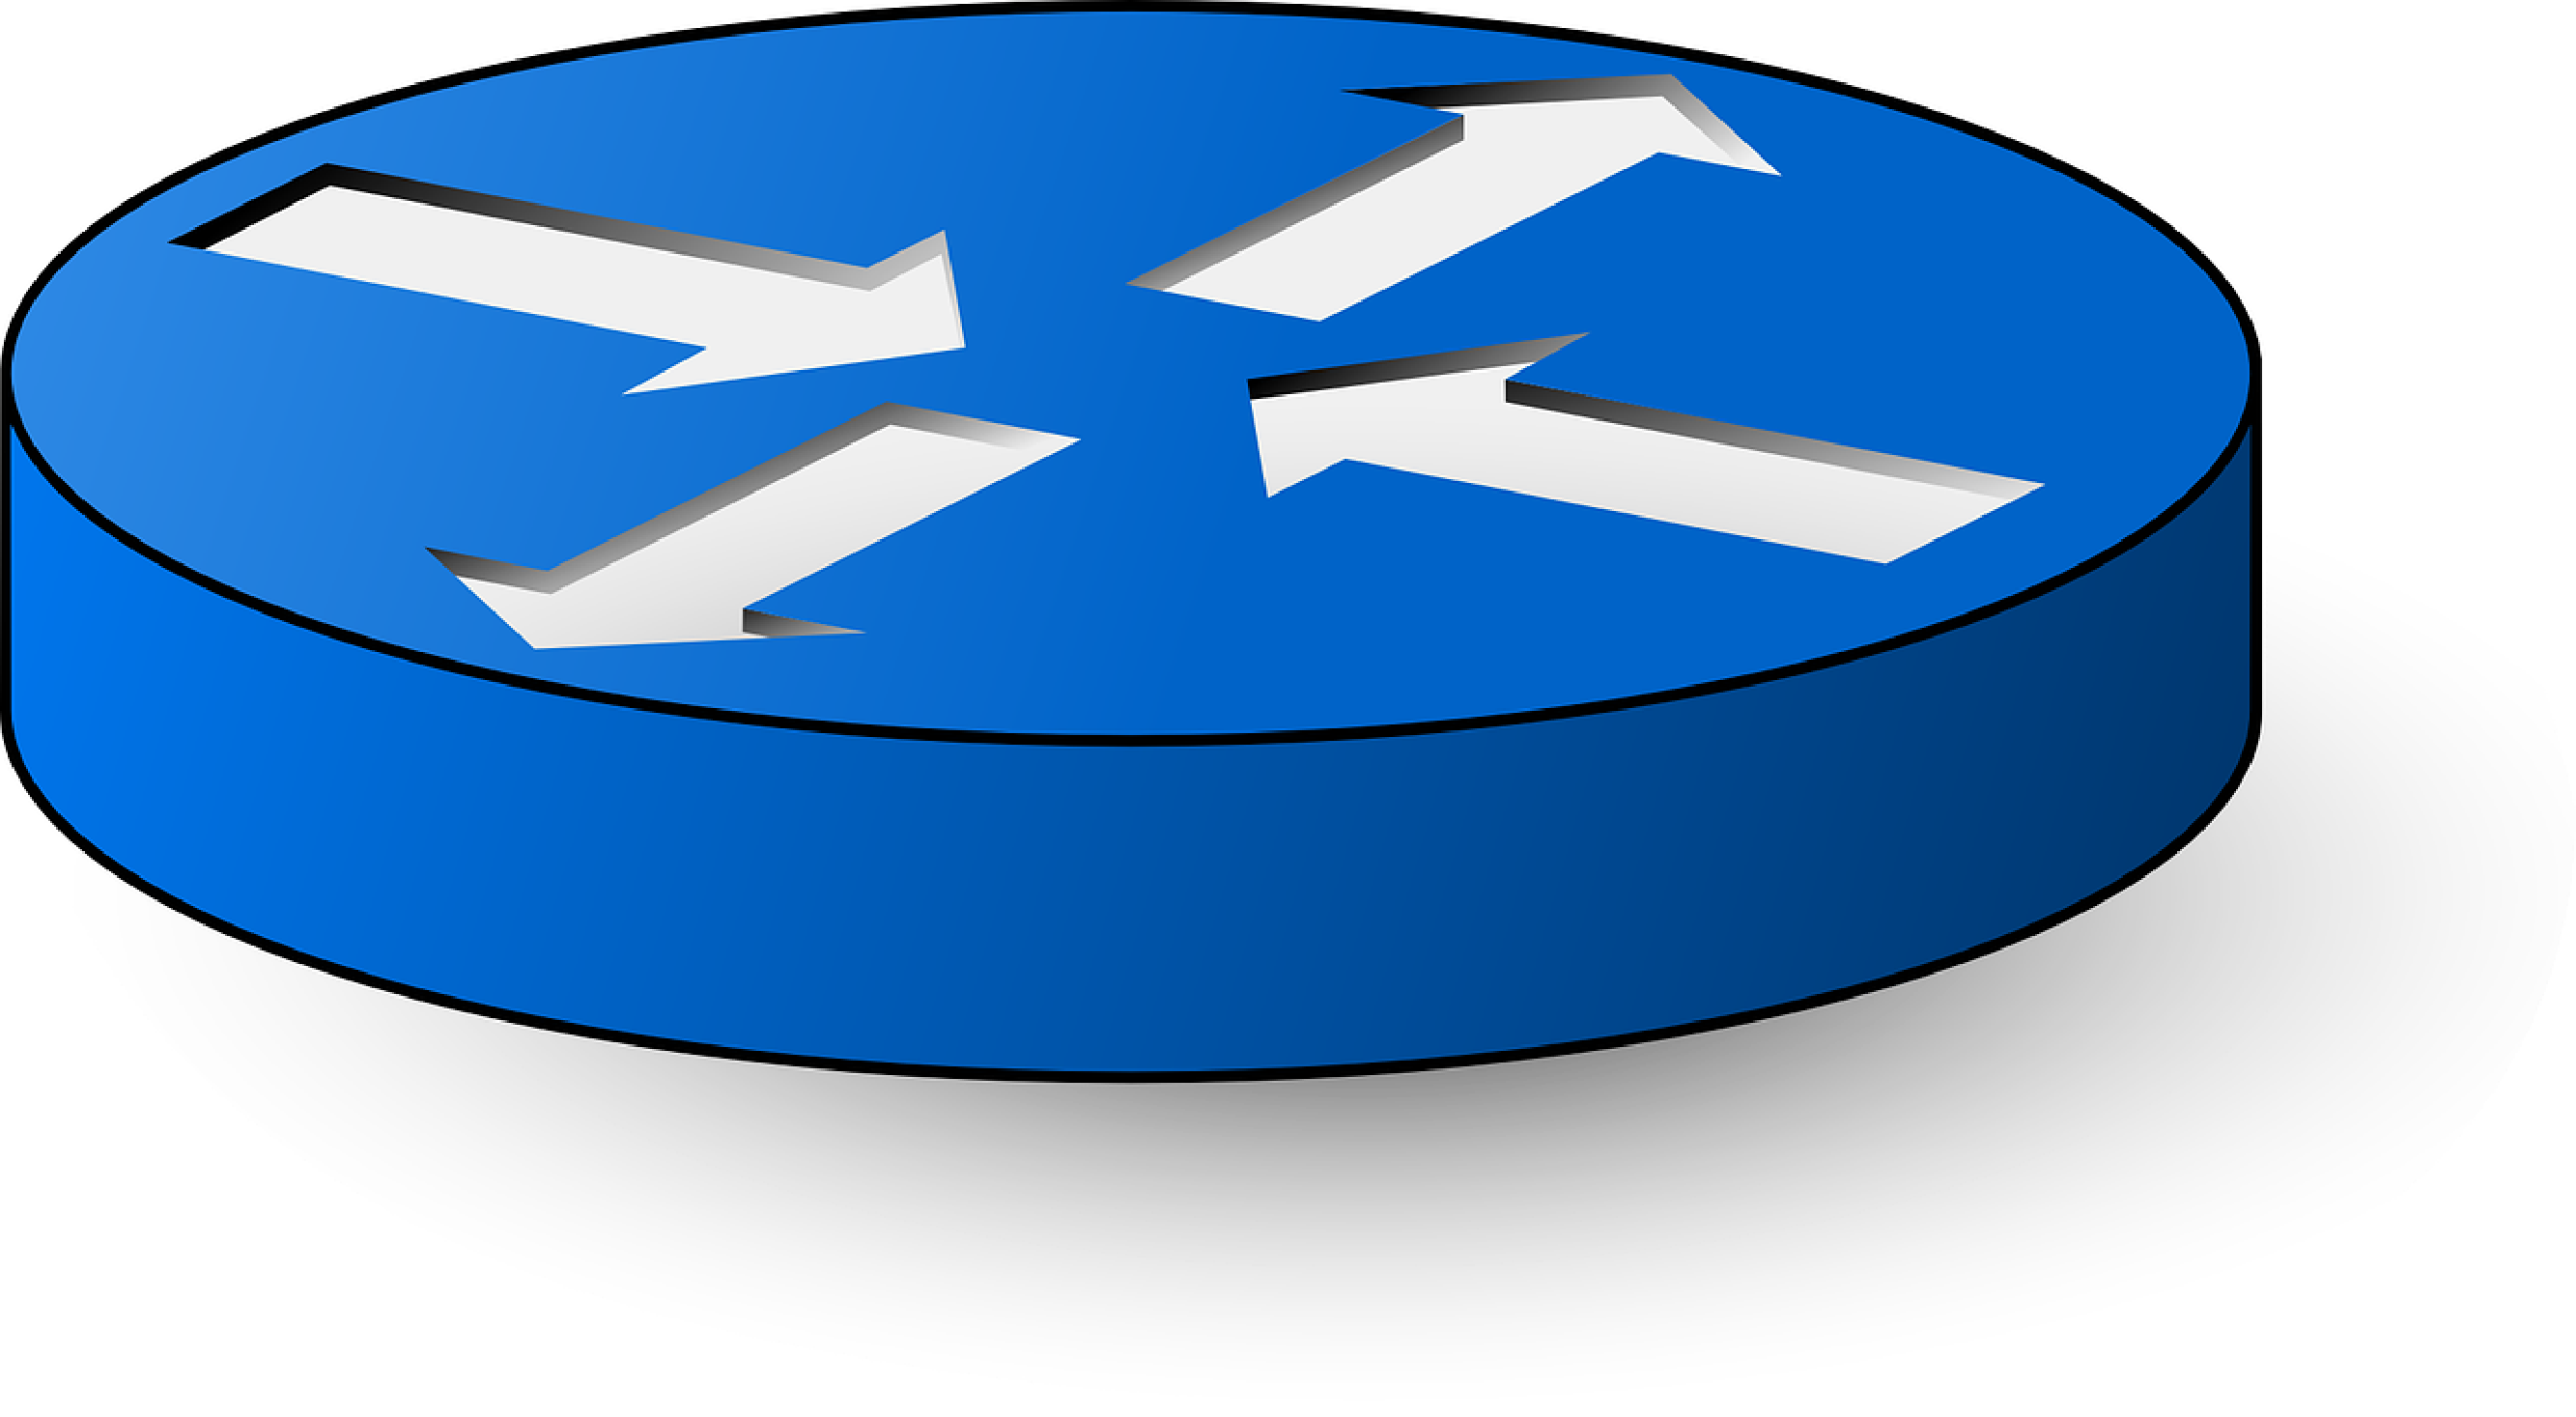
\includegraphics[width=52.5pt,height=52.5pt]{figures/router-30140_1280.pdf}};
%Straight Lines [id:da09222939335266478] 
\draw [color={rgb, 255:red, 74; green, 144; blue, 226 }  ,draw opacity=1 ][line width=1.5]    (236,313.33) -- (66.35,447.31) ;
\draw [shift={(64,449.17)}, rotate = 321.7] [color={rgb, 255:red, 74; green, 144; blue, 226 }  ,draw opacity=1 ][line width=1.5]    (14.21,-4.28) .. controls (9.04,-1.82) and (4.3,-0.39) .. (0,0) .. controls (4.3,0.39) and (9.04,1.82) .. (14.21,4.28)   ;

%Straight Lines [id:da6866328735169647] 
\draw [color={rgb, 255:red, 74; green, 144; blue, 226 }  ,draw opacity=1 ][line width=1.5]    (236,313.33) -- (432.28,405.56) ;
\draw [shift={(435,406.83)}, rotate = 205.17000000000002] [color={rgb, 255:red, 74; green, 144; blue, 226 }  ,draw opacity=1 ][line width=1.5]    (14.21,-4.28) .. controls (9.04,-1.82) and (4.3,-0.39) .. (0,0) .. controls (4.3,0.39) and (9.04,1.82) .. (14.21,4.28)   ;

%Shape: Cloud [id:dp2992812680460014] 
\draw  [fill={rgb, 255:red, 255; green, 255; blue, 255 }  ,fill opacity=1 ] (557.19,464.58) .. controls (556.29,457.33) and (559.25,450.16) .. (564.82,446.11) .. controls (570.39,442.05) and (577.58,441.82) .. (583.36,445.52) .. controls (585.4,441.31) and (589.14,438.4) .. (593.45,437.68) .. controls (597.76,436.95) and (602.13,438.5) .. (605.24,441.84) .. controls (606.98,438.02) and (610.4,435.46) .. (614.28,435.06) .. controls (618.17,434.65) and (621.97,436.47) .. (624.34,439.87) .. controls (627.48,435.82) and (632.49,434.11) .. (637.19,435.49) .. controls (641.89,436.87) and (645.44,441.08) .. (646.31,446.3) .. controls (650.16,447.45) and (653.38,450.37) .. (655.11,454.31) .. controls (656.85,458.25) and (656.94,462.82) .. (655.37,466.84) .. controls (659.17,472.24) and (660.06,479.44) .. (657.7,485.75) .. controls (655.35,492.05) and (650.11,496.52) .. (643.94,497.49) .. controls (643.9,503.41) and (640.93,508.84) .. (636.17,511.69) .. controls (631.42,514.54) and (625.63,514.36) .. (621.03,511.23) .. controls (619.07,518.32) and (613.56,523.53) .. (606.87,524.62) .. controls (600.18,525.71) and (593.52,522.48) .. (589.76,516.32) .. controls (585.16,519.36) and (579.63,520.23) .. (574.43,518.75) .. controls (569.23,517.27) and (564.8,513.55) .. (562.12,508.44) .. controls (557.42,509.04) and (552.87,506.37) .. (550.73,501.76) .. controls (548.6,497.16) and (549.33,491.58) .. (552.57,487.81) .. controls (548.37,485.11) and (546.23,479.75) .. (547.26,474.53) .. controls (548.29,469.31) and (552.26,465.41) .. (557.1,464.86) ; \draw   (552.57,487.81) .. controls (554.55,489.09) and (556.84,489.67) .. (559.13,489.47)(562.12,508.44) .. controls (563.11,508.31) and (564.07,508.04) .. (564.99,507.64)(589.76,516.32) .. controls (589.07,515.19) and (588.49,513.97) .. (588.04,512.7)(621.03,511.23) .. controls (621.39,509.94) and (621.62,508.6) .. (621.72,507.26)(643.94,497.49) .. controls (643.99,491.19) and (640.71,485.42) .. (635.52,482.66)(655.37,466.84) .. controls (654.53,468.99) and (653.24,470.89) .. (651.62,472.4)(646.31,446.3) .. controls (646.45,447.16) and (646.52,448.04) .. (646.5,448.93)(624.34,439.87) .. controls (623.55,440.87) and (622.91,442) .. (622.42,443.21)(605.24,441.84) .. controls (604.82,442.76) and (604.51,443.73) .. (604.31,444.73)(583.36,445.52) .. controls (584.58,446.3) and (585.71,447.24) .. (586.72,448.32)(557.19,464.58) .. controls (557.32,465.58) and (557.51,466.56) .. (557.78,467.53) ;
%Straight Lines [id:da885478252254038] 
\draw [line width=1.5]  [dash pattern={on 1.69pt off 2.76pt}]  (435.5,26.33) -- (474.5,26.83) ;


%Straight Lines [id:da6105591508346683] 
\draw    (435,42.71) -- (475,43.21) ;


%Straight Lines [id:da021279170004724568] 
\draw [color={rgb, 255:red, 74; green, 144; blue, 226 }  ,draw opacity=1 ][line width=1.5]    (438.5,75.13) -- (468.5,74.97) ;
\draw [shift={(471.5,74.96)}, rotate = 539.71] [color={rgb, 255:red, 74; green, 144; blue, 226 }  ,draw opacity=1 ][line width=1.5]    (14.21,-4.28) .. controls (9.04,-1.82) and (4.3,-0.39) .. (0,0) .. controls (4.3,0.39) and (9.04,1.82) .. (14.21,4.28)   ;

%Rounded Rect [id:dp201331626843132] 
\draw  [fill={rgb, 255:red, 217; green, 154; blue, 232 }  ,fill opacity=1 ] (6,276.78) .. controls (6,271.88) and (9.98,267.9) .. (14.89,267.9) -- (500.11,267.9) .. controls (505.02,267.9) and (509,271.88) .. (509,276.78) -- (509,303.45) .. controls (509,308.35) and (505.02,312.33) .. (500.11,312.33) -- (14.89,312.33) .. controls (9.98,312.33) and (6,308.35) .. (6,303.45) -- cycle ;

%Shape: Polygon Curved [id:ds08242749430225138] 
\draw  [color={rgb, 255:red, 255; green, 248; blue, 177 }  ,draw opacity=1 ][line width=2.25]  (41,423.33) .. controls (61,413.33) and (210,392.33) .. (232,407.33) .. controls (254,422.33) and (264,544.33) .. (248,574.33) .. controls (232,604.33) and (53.5,538.83) .. (33.5,508.83) .. controls (13.5,478.83) and (21,433.33) .. (41,423.33) -- cycle ;
%Straight Lines [id:da08659205633415445] 
\draw [color={rgb, 255:red, 255; green, 255; blue, 139 }  ,draw opacity=1 ][line width=2.25]    (435,91.71) -- (475,92.21) ;


%Straight Lines [id:da012161855616681594] 
\draw [color={rgb, 255:red, 242; green, 175; blue, 175 }  ,draw opacity=1 ][line width=2.25]    (435,111.71) -- (475,112.21) ;



% Text Node
\draw (55,213) node  [align=left] {(A1)};
% Text Node
\draw (211,471) node  [align=left] {(A3)};
% Text Node
\draw (113,594) node  [align=left] {Physical Infrastructure};
% Text Node
\draw (599,474) node  [align=left] {Internet};
% Text Node
\draw (417,171) node  [align=left] {(A2)};
% Text Node
\draw (587,501) node  [align=left] {(A4)};
% Text Node
\draw (521,26) node  [align=left] {Virtual Link};
% Text Node
\draw (528,47) node  [align=left] {Physical Link};
% Text Node
\draw (562,69) node  [align=left] {Hypervisor - Switch link};
% Text Node
\draw (548,92) node  [align=left] {vSDN1 Embedding};
% Text Node
\draw (549,113) node  [align=left] {vSDN2 Embedding};
% Text Node
\draw (257.5,290.11) node  [align=left] {Network Hypervisor};
% Text Node
\draw (55.76,67.79) node  [align=left] {{\small vSDN1}};
% Text Node
\draw (282.98,171.5) node [scale=0.9] [align=left] {{\small vSDN2}};


\end{tikzpicture}

\caption{Attack surface of the SDN environment}
\label{fig:attack-surface}
\end{figure}

%\GB{I suggest: ``Attacks against Migration'' as a title}
\label{sec:attacker-model}
The migration of a VN creates virtual nodes and virtual links between them.
Thus, based on  the migration functions we introduced in Section~\ref{sec:migration} and the axioms we have presented in Section~\ref{sec:prop-conf}, we will describe the different components of a threat using the following syntax
%\GB{terms?}
%\FC{The syntax is the combination of terms}
: Attacker - Action - Target.

\subsubsection{Attacker}
We consider the different locations from where an attacker could attack the migration of the VN. 
Figure~\ref{fig:attack-surface} places four different attackers: the insider (A1), the collocated user (A2), the provider (A3), the outsider (A4).

The insider is an attacker located inside the VN that is going to be migrated.
It can be a malicious user able to control a virtual node and deploy incorrect flow rules.
The collocated user is another user of the virtualization platform.
He can use his own topology on the physical infrastructure.
The provider is the owner of the physical infrastructure.
He has access to the SDN switches embedding the virtual topologies.
The outsider is a malicious user outside the SDN environment.
He has limited access to both the VNs and the physical infrastructure.

\subsubsection{Action}
There are 4 major actions that can be performed by an attacker to affect the VNs and their environment.
The first two are related to the infrastructure and the others are related to the data carried across the network.
\begin{itemize}
\item Unauthorized access to a network element.
\\ This type of access represent a violation of each security property.
\item Disruption of service on a network element.
\\ The availability of physical and virtual resources becomes compromised
\item Information disclosure without authorization.
\\ The confidentiality of the data is affected
\item Information modification or destruction without authorization.
\\ The integrity of the data or the network resource is affected
\end{itemize}

\subsubsection{Target}
We can consider two types of targets: nodes or data.
The nodes are either the physical switches in the infrastructure or the virtual nodes of a VN.
There are three types of data inside a VN and its infrastructure.
The user data carried by the virtual elements, the management data and the configuration data carried by the infrastructure. 

The user data is the traffic generated by the user and going through the VN.
The management data is made of the different packets exchanged between the virtualization layer and the physical infrastructure to operate properly (capacities, established links, etc.).
The configuration data are the different flow rules deployed on the physical switches when instantiating a VN.
It is important to note that both configuration data and management data are issued by the hypervisor but do not serve the same purpose nor have the same frequency of use, even though they use the same communication channel.
Management data are regularly exchanged between the hypervisor and the switch to maintain the view of the infrastructure (\eg symmetric messages like HELLO requests), while configuration data are sent when installing new flow rules or removing old ones (asynchronous messages sent because of flow expiration).

\begin{table}[h]
\centering
\begin{tabular}{|l|l|l|}
\hline
\textbf{Attacker}   & \textbf{Action}    & \textbf{Target}             \\ \hline
Insider    & Unauthorized access                  & Nodes              \\ \hline
Collocated & Disruption of service                & User data          \\ \hline
Provider   & Information disclosure               & Management data    \\ \hline
Outsider   & Information modification/destruction & Configuration data \\ \hline
\end{tabular}
\caption{Elements of the attack model}
\label{tab:attack-model}
\end{table}

\subsubsection{Attacks}
\label{sec:model-attacks}
%\GB{please in this section and the following, specify which attack is directed against which algorithm}
In the previous sections, we have defined the different attackers, as well as the malevolent actions and possible targets in the virtualization infrastructure. 
Table~\ref{tab:attack-model} summarizes these information.
We will combine elements from each column together to define several attacks targeting the migration process or the user's data.
These attacks are based on two assumptions: a stable initial environment and no outsider attacker.
We consider that the virtualization infrastructure is not already under attack when a malicious user decides to launch one of the following attacks.
This assumption comes from the fact that we aim to detect the switch between a safe state and a compromised state. From a practical point of view, the infrastructure runs most of the time with a normal behavior.
We also assume that an attacker residing outside the virtualization infrastructure and not using the virtualization service has little to no attack surface on the infrastructure.
Most interfaces to interact with any component of the system are limited in visibility from the outside world.
For instance, the DPAC provides an interface for end users to interact with their virtual network, and there is no openly identified weaknesses for an outsider to use (\ie the hypervisor will reject commands from unauthorized users).
Similarly, the CPAC provides an interface between the hypervisor and the physical nodes, and there is no functional use for this component to be interfaced with the outside world.
We summarize the attacks in Table~\ref{tab:use-case-attack}.

% Please add the following required packages to your document preamble:
% \usepackage{graphicx}
\begin{table}[h]
\resizebox{\textwidth}{!}{%
\begin{tabular}{|l|l|l|l|l|}
\hline
Attack                   & Attacker        & Action                      & Target                   & Summary                                                                  \\ \hline
Denial of Service        & Provider side   & Service disruption          & Nodes                    & Resource depletion (DNS amplification ICMP flood) \\ \hline
Info. Disclosure   & Collocated user & Info. disclosure   & Node, user data          & Data exfiltration by malicious flow rules injection    \\ \hline
Config. alteration & Provider side   & Info. modification & Node, config. data & Man-in-the-middle attack to Modify config. data             \\ \hline
Denial of Service        & Provider side   & Service disruption          & Nodes                    & Resource depletion (DNS amplification ICMP flood) \\ \hline
\end{tabular}%
}
\caption{Use cases: Attacking the migration}
\label{tab:use-case-attack}
\end{table}
% In this paper, we chose to focus on the security aspects of the confidentiality.
% Thus, we are more interested in the unauthorized access and information disclosure of the attack model.
% As we also consider a stable initial environment, an outsider attacker is too limited to attack the infrastructure and is therefore of no interest in this paper.
% Finally, the different data present in the threat model are similar enough in essence.
% Attacking one or another makes no difference in terms of formal modeling.
% We propose two different attacks, one focusing on the disclosure of confidential traffic carried by a VN, and the other will be an on-site attack on a physical node.
%\GB{please specify which migration algorithms are attacked here, and in the next section}

%\GB{in general, you could sum up in a table what attacker can do what against what. I am surprised that you only have two scenarios. Usually attacker classes tend to be ordered sets. But it is not always the case}
%\FC{I believe one attack scenario per migration algorithm is enough. However I agree with the table, will work on it today. I don't understand what you mean by ordered sets.}
%\GB{usually, you describe different attackers that share abilities, from the least potent to the most potent. Usually the least potent has ability to perform action A, then the second least potent can do actions A and B, then another can do actions A, C and D, and the most potent can do A, B, C and D. If you are presenting only a couple of scenarios, you may actually list all possible scenarios, \ie triplets (Attacker, Action, Target) and explicitly state that you will only demonstrate two of them, motivating why you choose these}




\paragraph{Denial of Service}\textbf{\\}
In this scenario, the attacker is located inside the physical infrastructure, and will launch Denial of Service (DoS) attacks to render one or several nodes unavailable.
This will result in a forced migration, thus creating an opportunity to compromise the migration process.
This attack becomes the necessary first step of all of the following attacks.

\subparagraph{Hypotheses}\textbf{\\}
% \textbf{Location:} The attacker is located either inside the physical infrastructure or is a malicious user of the virtualization service.\\
\textbf{Information gathering}\textbf{\\}
THe attacker has collected information about his victim, and how to precisely target network equipments.
The information collection process is considered out of scope of this work.\\
\textbf{Traffic generation:} The attacker can generate enough traffic to cause a service disruption.
DoS attacks like ICMP flood or DNS amplification are used for to deplete network resources in the infrastructure.

\subparagraph{Attack methodology}\textbf{\\}
The attacker will generate massive amounts of traffic to generate congestion effects inside the network. The attacker may be located inside the physical network, or he may be the owner of a Virtual Network. The second option is easier to achieve but the attacker will be confronted to the resource isolation enforced by the hypervisor (\ie FlowVisor bandwidth isolation mechanism)


\subparagraph{Impacts}\textbf{\\}
This attack impacts the following security properties:\\
The \textbf{availability} of nodes in the infrastructure has been impacted because of the DoS attack.
% \begin{itemize}
%     \item $node\_availability(N)$
%     \item $vnode\_availability(n)$
%     \item $vlink\_availability(l)$
%     \item $path\_availability(P)$
%     \item $vpath\_availability(P)$
% \end{itemize}

\paragraph{Information disclosure}\textbf{\\}
In this scenario, the attacker is a collocated user that is gaining access to another user's confidential traffic. 
\subparagraph{Hypotheses:}\textbf{\\}
\textbf{Collocated attacker:} The attacker owns a virtual network in the infrastructure.\\
\textbf{Migration trigger:} The attacker can trigger the migration of the victim's VN.\\
\textbf{Embedding knowledge:} The attacker has approximate knowledge of the new substrate network.\\
\textbf{Writing rights:} The attacker can install specific flow rules inside a node.

\subparagraph{Attack methodology:}\textbf{\\}
In order to gain access to confidential data, the attacker generates instability in the infrastructure. Typically, generating lots of requests between nodes and users will create enough disruption to force the migration.
Then, he will use his knowledge of the embedding of the virtual network to target specific nodes.
Deploying probes in the network or attacking on a large scale the infrastructure could lead the virtualization layer to a particular deployment. Co-residency-based attacks and vulnerabilities are exploited in several cases~\cite{malicious-atya2017,nomad-Moon2015b,getoffmucloud-Ristenpart2009,stalling-atya2017}.
An attacker uses time-based attacks to verify the co-residency with his victim and then the attacker will compromise the confidential data by redirecting it from the victim's VN toward a malicious end host belonging to him.
Such attacks rely on deploying specific flow rules on a set of physical nodes that will copy the confidential traffic and route it towards the attacker.
This methodology is illustrated in~\cite{Costa2015,Sphinx-Dhawan2015}.


\subparagraph{Impacts}\textbf{\\}
This attack impacts the following security properties:\\
The \textbf{availability} of specific nodes in the infrastructure has been impacted to force the migration.
% \begin{itemize}
%     \item $node\_availability(N)$
%     \item $vnode\_availability(n)$
%     \item $vlink\_availability(l)$
%     \item $path\_availability(P)$
%     \item $vpath\_availability(P)$
% \end{itemize}
The \textbf{confidentiality} of the data that has been extracted by the attacker.
% \begin{itemize}
%     \item $confidentiality(D)$
% \end{itemize}
The confidentiality of the nodes is not impacted because the attacker did not access the node by installing flow rules on them, with respect to the definition provided in the previous section.\\
The \textbf{integrity} of the different nodes that have been used to forward the data to the attacker.
%     \begin{itemize}
%     \item $node\_integrity(N)$
%     \item $vnode\_integrity(n)$
%     \item $vlink\_integrity(l)$
% \end{itemize}
The \textbf{co-residency} between both victim and attacker VNs has been increased for the attacker to successfully exfiltrate the victim's data.


\paragraph{Migration alteration}\textbf{\\}
We now consider a malicious user intending to exploit the migration process to modify the configuration deployed on a node.

\subparagraph{Hypotheses:}\textbf{\\}
\textbf{Provider side attacker:} The attacker sits between the node and the hypervisor.\\
\textbf{Man-in-the-middle:} The attacker can modify the configuration information sent by the hypervisor in a specific node.\\
\textbf{Migration trigger:} The attacker can trigger the migration of the victim's VN.\\
\textbf{Embedding knowledge:} The attacker has approximate knowledge of the new substrate network.

\subparagraph{Attack methodology:}\textbf{\\}
First of all, the attacker gains access to a networking equipment between the target node and the hypervisor. Similarly to the previous attack, this is done by exploiting vulnerabilities in the physical equipments.
Then, he will trigger the migration of a specific physical node, that will be redeployed on the node targeted by the Man-in-the-middle attack.
Once the hypervisor sends the different flow rules, the attacker will modify them to fit his extraction scheme.

\subparagraph{Impacts:}\textbf{\\}
This attack impacts the following security properties:\\
The \textbf{availability} of the attacked node has been impacted to trigger the migration.
% \begin{itemize}
%     \item $node\_availability(N)$
%     \item $vnode\_availability(n)$
%     \item $vlink\_availability(l)$
%     \item $path\_availability(P)$
%     \item $vpath\_availability(P)$
% \end{itemize}
The \textbf{confidentiality} of the configuration data that has been modified by the attacker.
% \begin{itemize}
%     \item $config\_confidentiality(conf)$
% \end{itemize}
The confidentiality of the nodes is not impacted for the same reasons described in the previous attack.\\
The \textbf{integrity} of the node and its configuration has been compromised
%     \begin{itemize}
%     \item $node\_integrity(N)$
%     \item $vnode\_integrity(n)$
%     \item $vlink\_integrity(l)$
%     \item $config\_integrity(conf)$
% \end{itemize}

% 
